\documentclass [11pt, letterpaper] {article}
\input {headings}
\newcommand \recipeName {Grilled Ratatouille}
\newcommand \fileName {GrilledRatatouille}
\chead {\recipeName}

\begin {document}
\input {title}

Years ago I was attending an academic conference in Lyon in France. One evening, I was dining by myself and sat down on a sidewalk table in a non-descriptive restaurant on a street with a row of such restaurants. I ordered a simple small steak and when picking side dishes, I casually selected the ratatouille. It was a revelation. This recipe is inspired on that simple side dish from that simple sidewalk restaurant. This is an adaptation of the recipe for Grilled Ratatouille Provencal from the book {\em The New Professional Chef --- The Culinary Institute of America} editado por Mary Deirdre Donovan, 8th edition, 1996. This adaptation makes it very easy to make a very large batch for a large party. The best result is achieved by preparing the infused olive oil, braised onions and tomato sauce two days before the party. Then grill the vegetables and mix into the tomato sauce the day before. Keep the Ratatouille in the refrigerator overnight. The day you will serve it, remove from the fridge early to allow it come come back to room temperature. You can gently warm it up in a 180F oven to serve it lukewarm.
\vspace{0.5in}

\begin{description}

\item[Ingredients:]\ \\
	\begin{itemize}
	\item 25 cloves of garlic (peeled)
	\item 8 sprigs of rosemary
	\item 500 ml Extra-virgin olive oil
	\item 3 large onions (preferably sweet Vidalia onions, but yellow onions are also ok)
	\item 2 large cans of tomatoes (good quality Italian canned tomatoes) 
	\item 1 small jar of roasted and peeled red bell peppers (or three fresh red bell peppers that you roast and peel yourself) 
	\item 1 hot pepper (if in Brazil, use two pimenta de cheiro)
	\item Freshly ground black pepper
	\item Fresh Basil (or fresh Italian Parsley)
	\end{itemize}

\item[Procedure:]\ \\
	\begin{enumerate}
	\item {\bf Rosemary-Garlic Infuse oil}
	\begin{itemize}
	\item Put olive-oil in a shallow saucepan.
	\item Slice five cloves of garlic in half and add to the oil.
	\item Add rosemary sprigs.
	\item Put on stove at very low heat until it is fairly warm, but not frying the garlic.
	\item Let it cool off and put in a jar.
	\item Can be stored in a cool place for a couple of days until you are ready to proceed with the recipe.
	\end{itemize}
	\item {\bf The following two steps can be done two or three days in advance.}
	\item {\bf Tomato Sauce}
	\begin{itemize}
	\item Turn oven to 300 F (150 C)
	\item Open the tomato cans. 
	\item Pour 1/3 of a cup of the infused oil in a non-reactive heavy-duty saucepan that has a lid and can go into the oven.
	\item Slice three cloves of garlic in half and add to the saucepan.
	\item Add the diced hot pepper (or the two pimento de cheiro) to the saucepan.
	\item Put the pan over moderately high heat and cook just until the garlic turns pale brown --- do not overcook.
	\item Dump the cans of tomato into the pan to cool off the garlic/oil mixture and prevent overcooking the garlic.
	\item Sprinkle with a small amount of salt and bring the tomato to a gentle simmer.
	\item Place in the 300 F oven and bake it covered for two hours, stirring it every 45 minutes or so.
	\item After two hours add the diced roasted peppers, with their juices, to the saucepan.
	\item Bake for another hour.
	\item {\bf Note:} If using fresh ripe tomatoes, you can simply wash and dump the whole tomatoes into the pot. Later you can pass the sauce through a food mill at the large-hole screen to remove the tomato peels.
	\end{itemize}
	\item {\bf Braised Onions with Garlic}
	\begin{itemize}
        		\item Peel the onions and cut them into a large dice
		\item Put the diced onions on an oven-proof dish with cover 
		\item Add three tablespoons of the infused olive oil to the dish
		\item Add the remaining cloves of garlic (whole) to the dish.
		\item Lightly sprinkle with salt.
		\item If using yellow onions, sprinkle with 1/2 teaspoon of sugar.
		\item Sprinkle with freshly ground pepper.
		\item Toss the onions, cover the dish and put in a 300 F (150C) oven for about three hours, tossing the onions about every 45 minutes or so --- the onions and the tomato sauce bake at the same time.
		\item They are done when they are soft, reduced volume significantly and are lightly browned on some some of the edges.
		\item Mix the braised onions into the cooked tomato sauce.
		\item Remove from the oven, let it cool and put into a closed container and put in the refrigerator.
	\end{itemize}
	\item {\bf Grilling the Vegetables}
	\begin{itemize}	
		\item  Slice the eggplants lengthwise into thick slices (about 3/4 inch thick).
		\item Lightly sprinkle the slices with salt on both sides (careful to not oversalt them because they will reduce in volume after grilled).
		\item Let the salted eggplants stand on a bowl or colander for at least half an hour.
		\item Do the same process for the zucchini (slice, lightly salt, let it stand).
		\item Get your grill as hot as you can (my gas grill gets to 550F)
	 	\item Brush the grill with a hard grill brush to make sure it is clean
	 	\item Pour a small amount of oil in a small dish, fold a piece of paper towel several times and holding the folded paper towel with kitchen tongues, deep it in the oil and smear all over the grill. Cover the grill to let the oil burn for a minute. Repeat the process three or four times to reduce the stickiness of the grill. 
		\item Reduce the temperature of the grill to a moderate high heat.
		\item Dry the slices of eggplant  with paper towels.
		\item Pour some of the garlic-infused olive oil into a dinner plate.
		\item Quickly coat both sides of each eggplant slice on the olive oil in the plate. Keep adding more oil to the plate as you need. You may want to coat as many slices as will fit in your grill before you start grilling.
		\item Grill the eggplants until they are soft flipping them with a metal spatula as needed. 
		\item When removing from the grill put in a covered bowl so that they continue cooking as they cool down.
		\item Repeat the process (pat dry, coat with garlic-infused oil, and grill) with the zucchini.
		\item When they are cool enough to handle, cut the grilled vegetables into a large dice.
		\item Gently mix the diced grilled vegetables, along with any juices that they have released, into the tomato sauce.
		\item Put back into the refrigerator and keep it overnight.
	\end{itemize}
	\item{\bf Basil and Serving}
	\begin{itemize}	
		\item On the day you are serving, remove from the fridge several hours before serving to allow it to come close to room temperature.
		\item Chop the basil and mix into the ratatouille.
		\item Add freshly ground pepper to the ratatouille (to taste).
		\item Put the ratatouille into an 180F oven until you are ready to serve.
	\end{itemize}	
     	\end{enumerate}         
\end{description}
\begin{table}
\begin{tabular}{cccc}
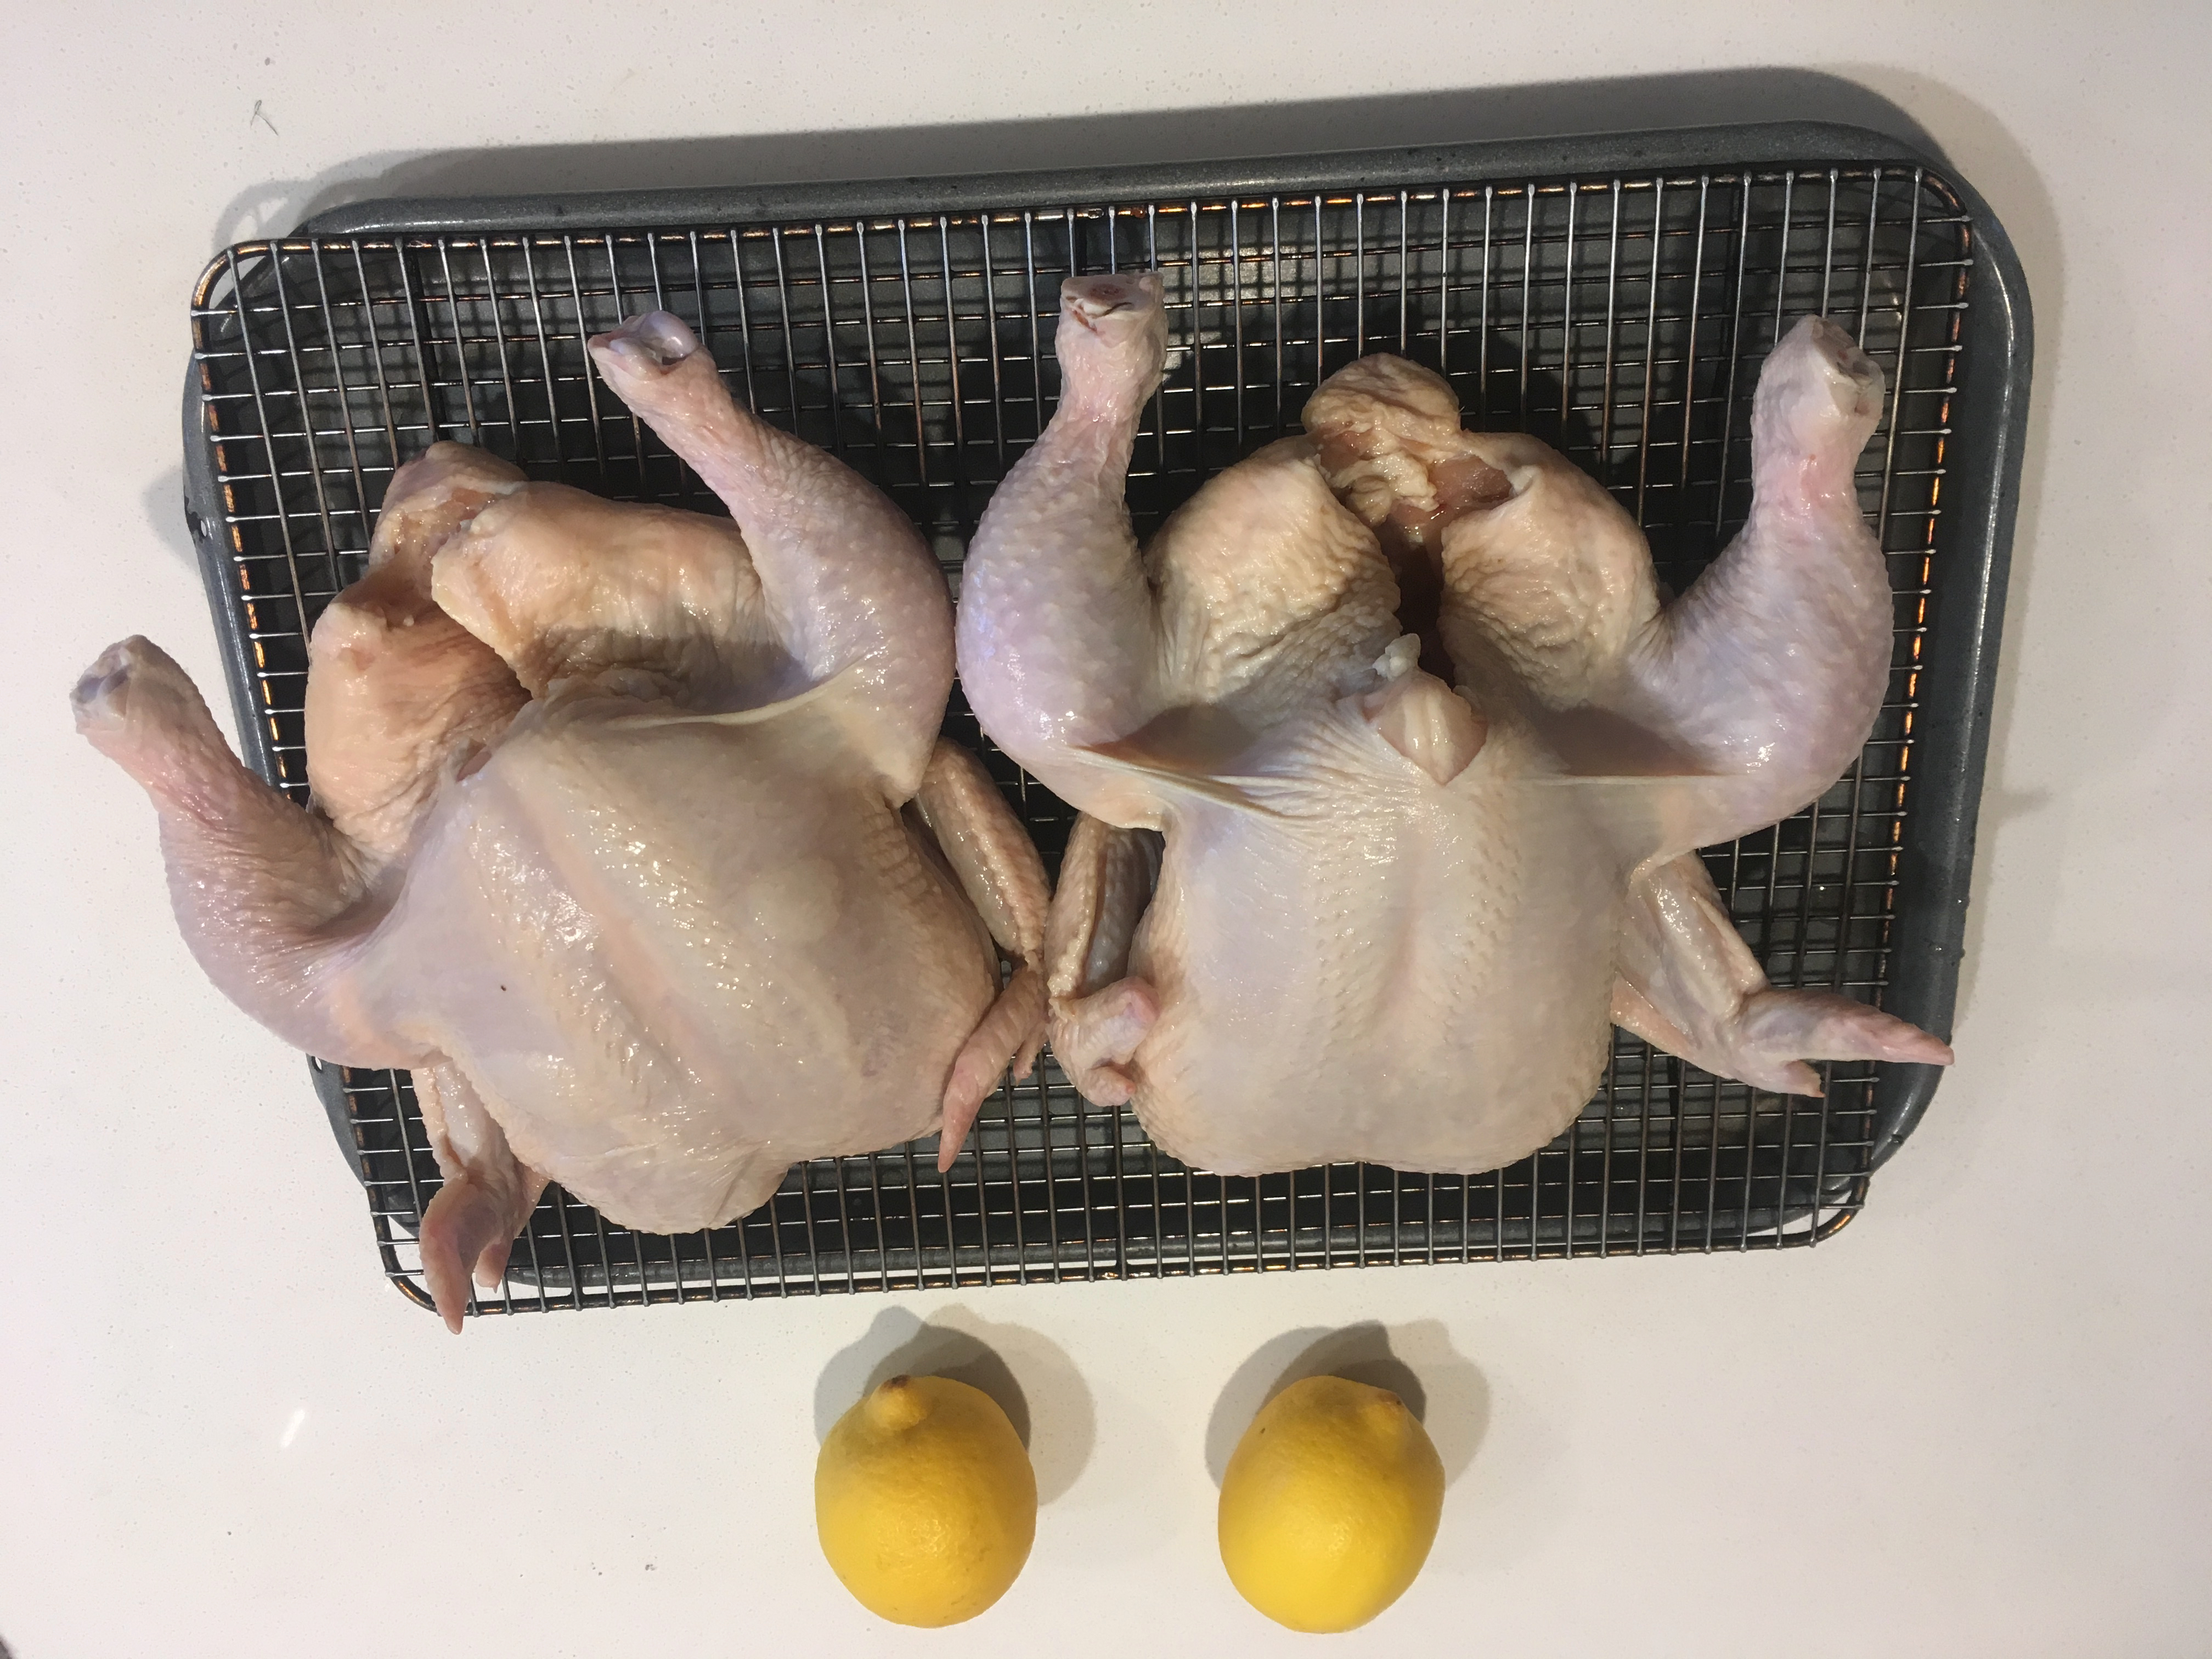
\includegraphics[width=0.25\textwidth]{\imageDir/\fileName/IMG_3197.jpg} &
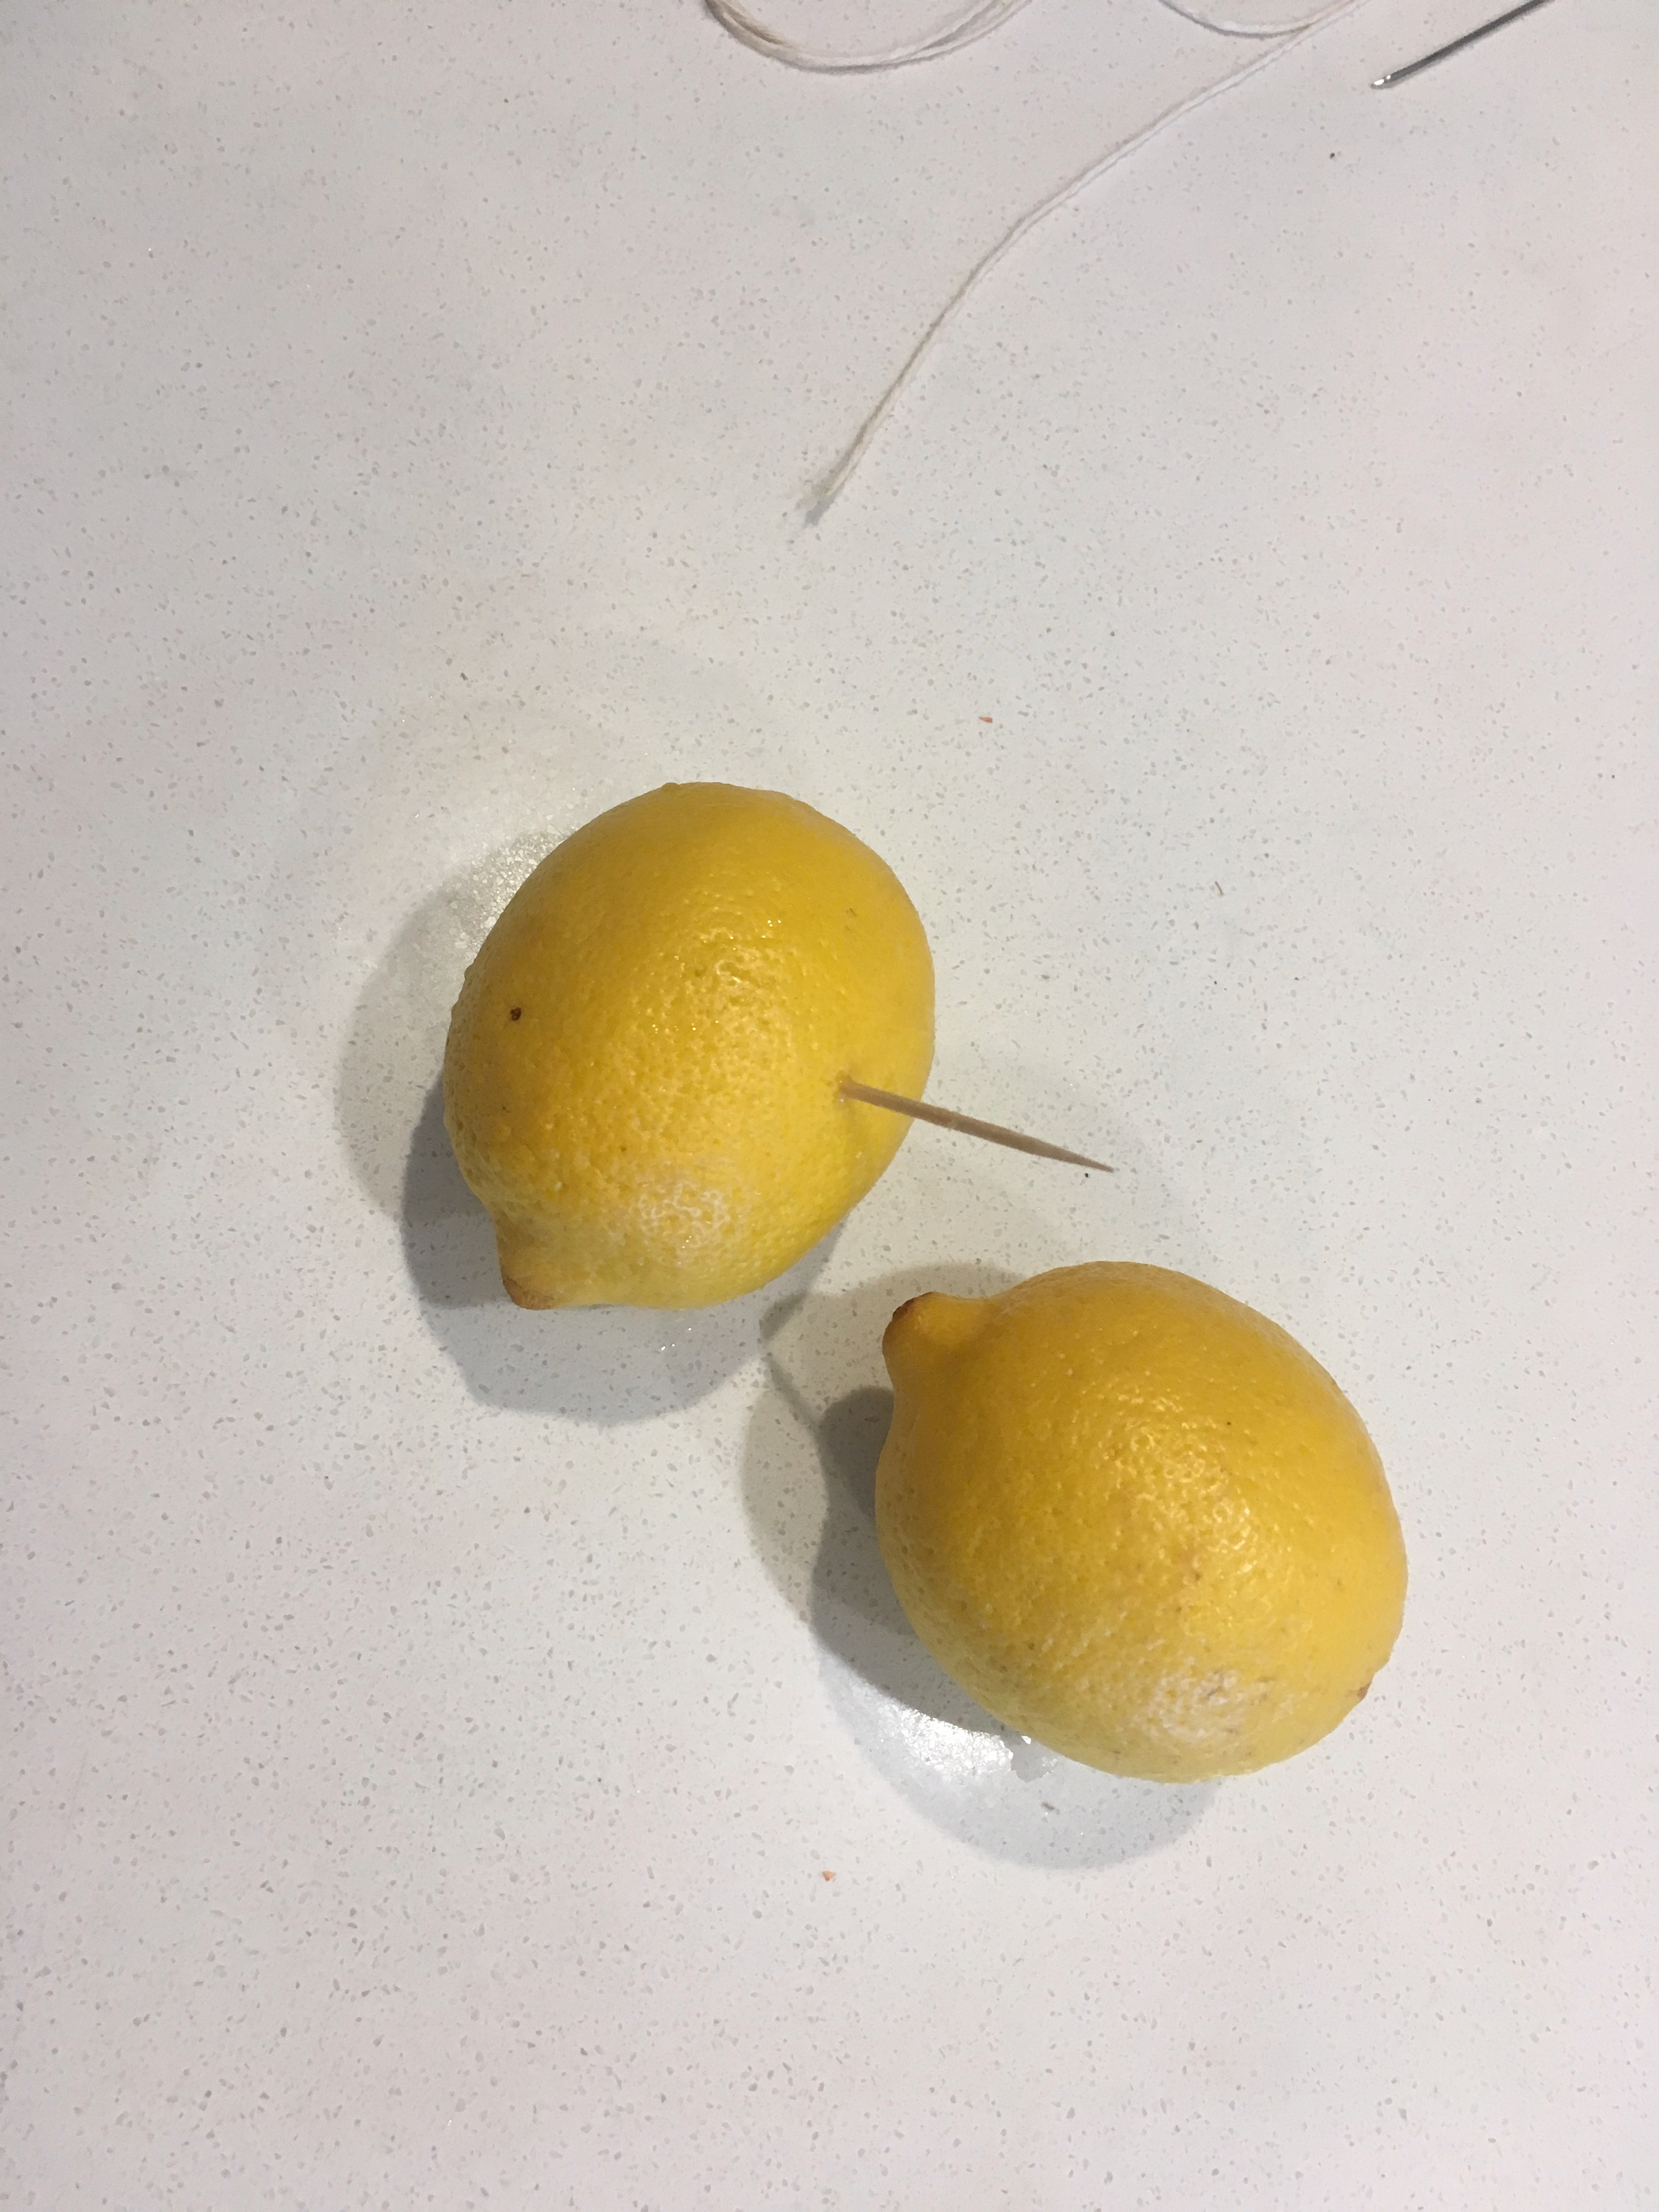
\includegraphics[width=0.25\textwidth]{\imageDir/\fileName/IMG_3212.jpg} &
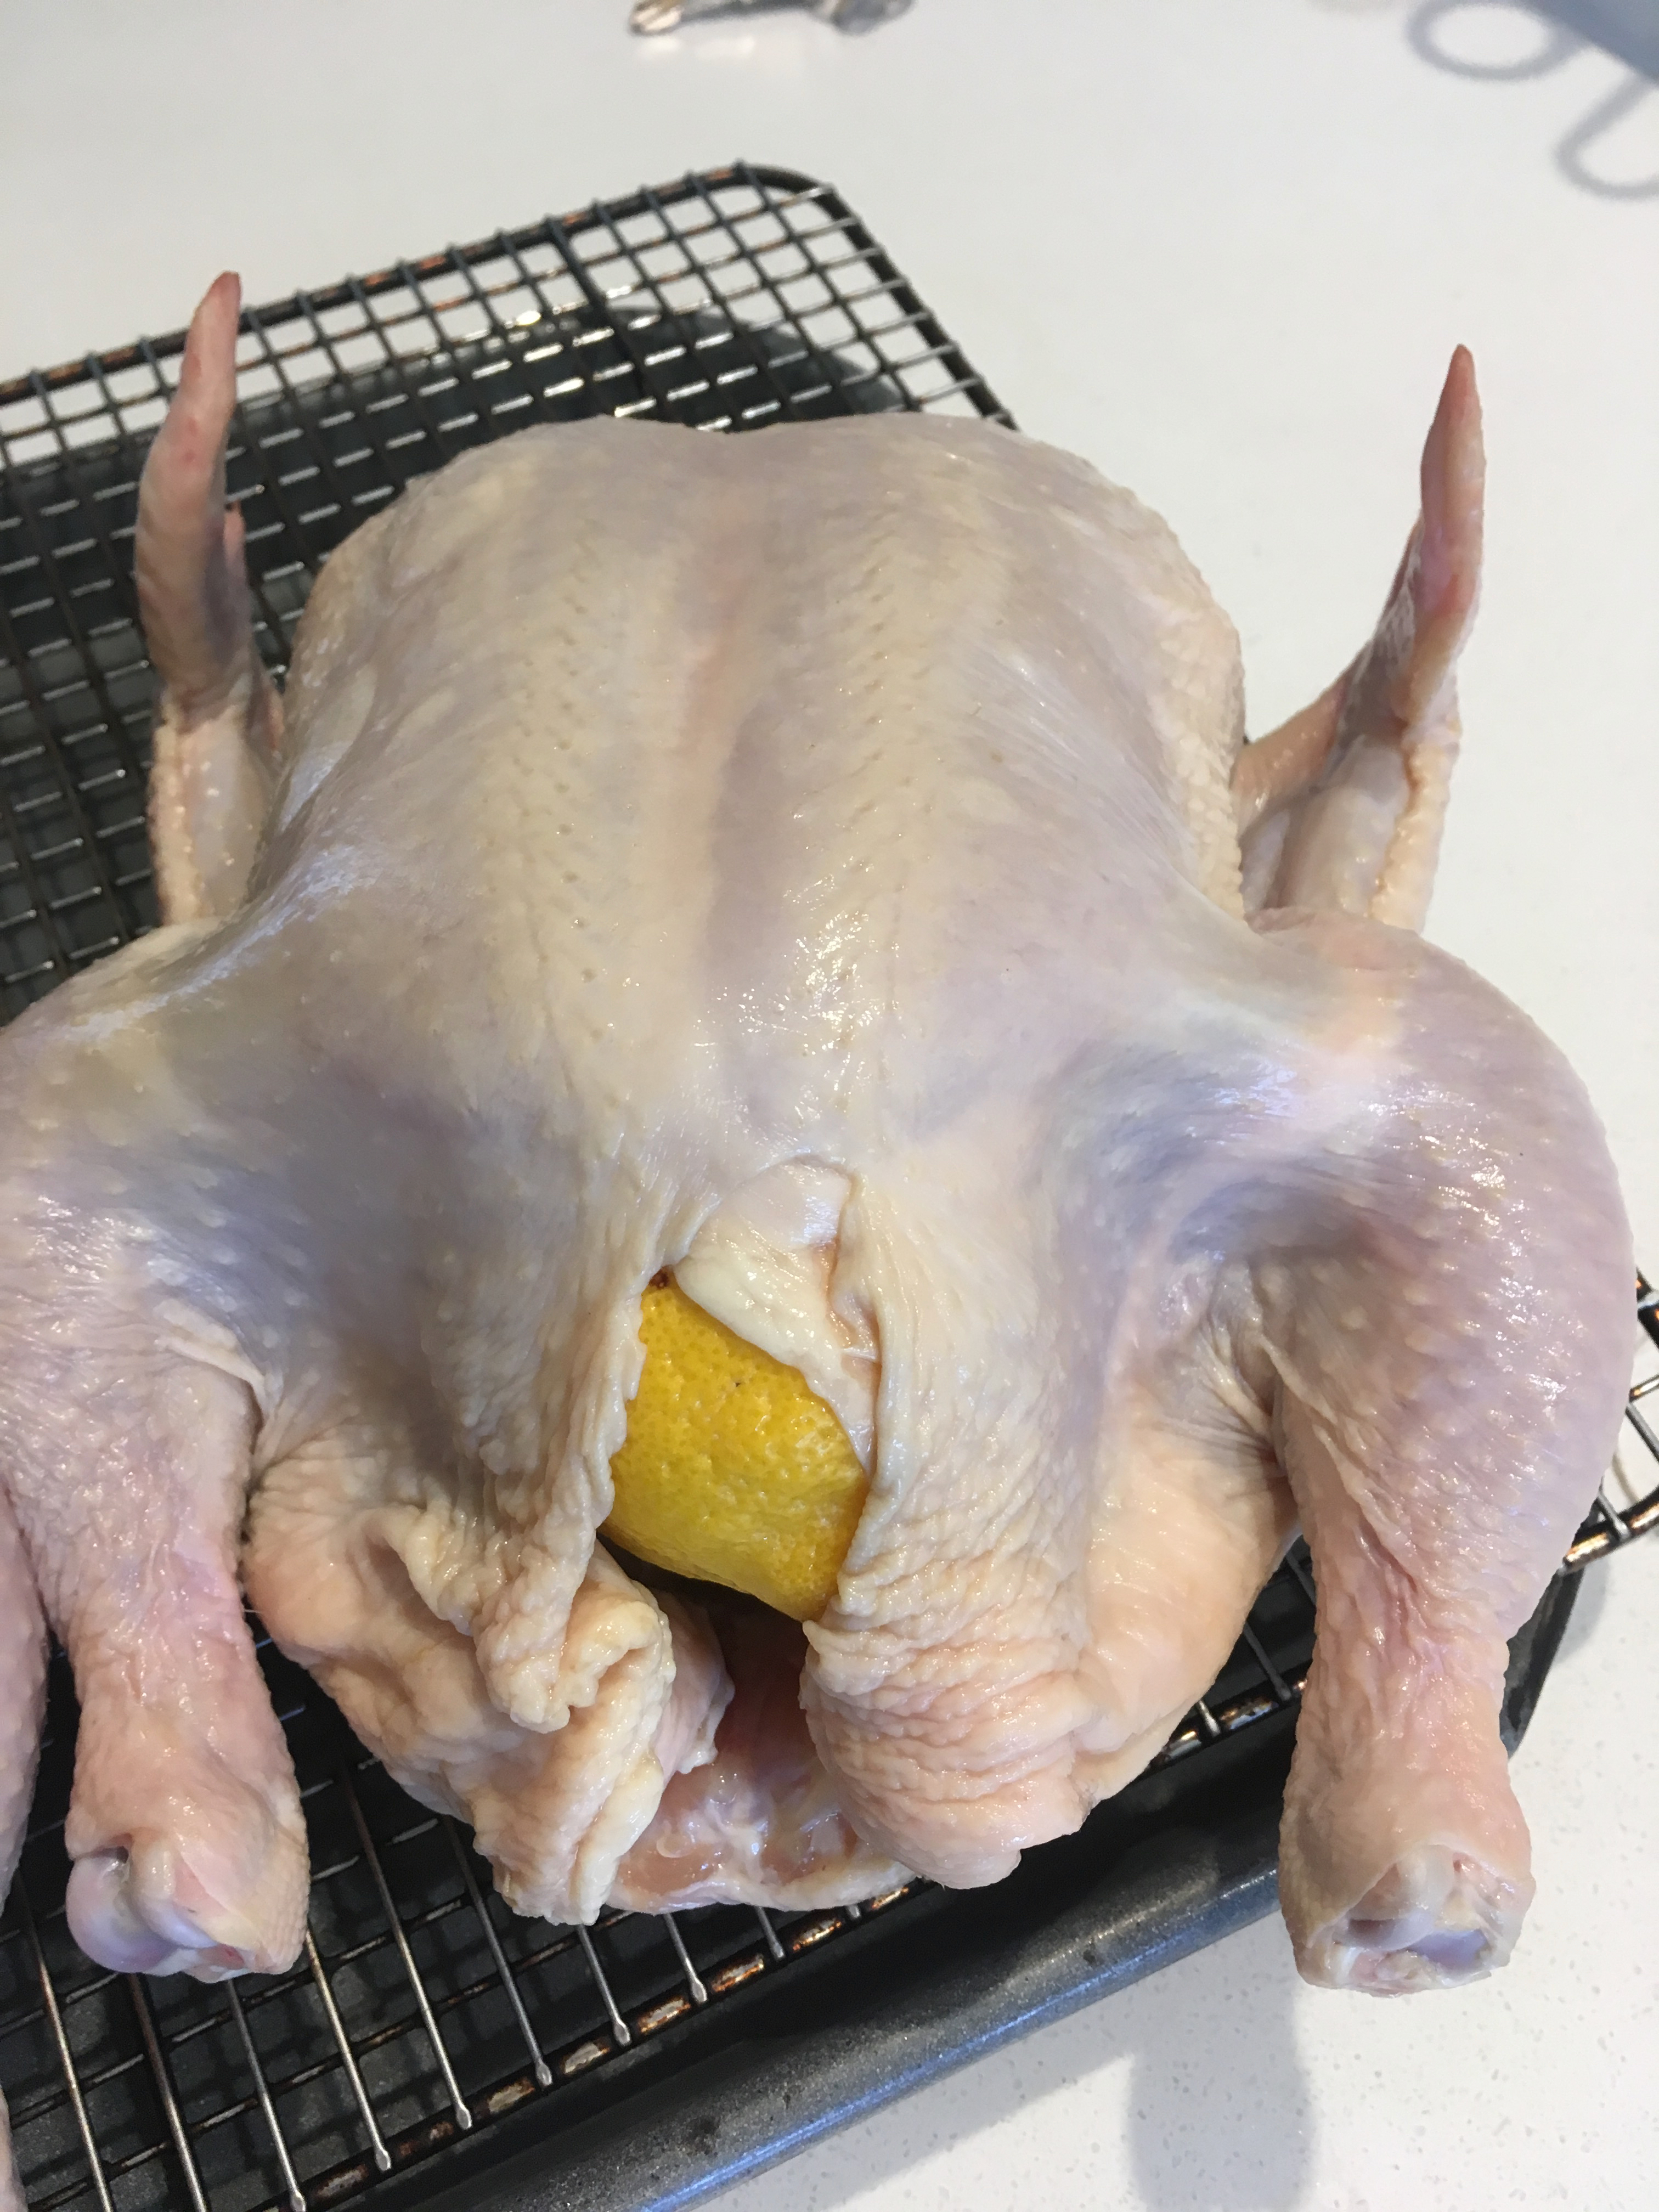
\includegraphics[width=0.25\textwidth]{\imageDir/\fileName/IMG_3213.jpg} \\
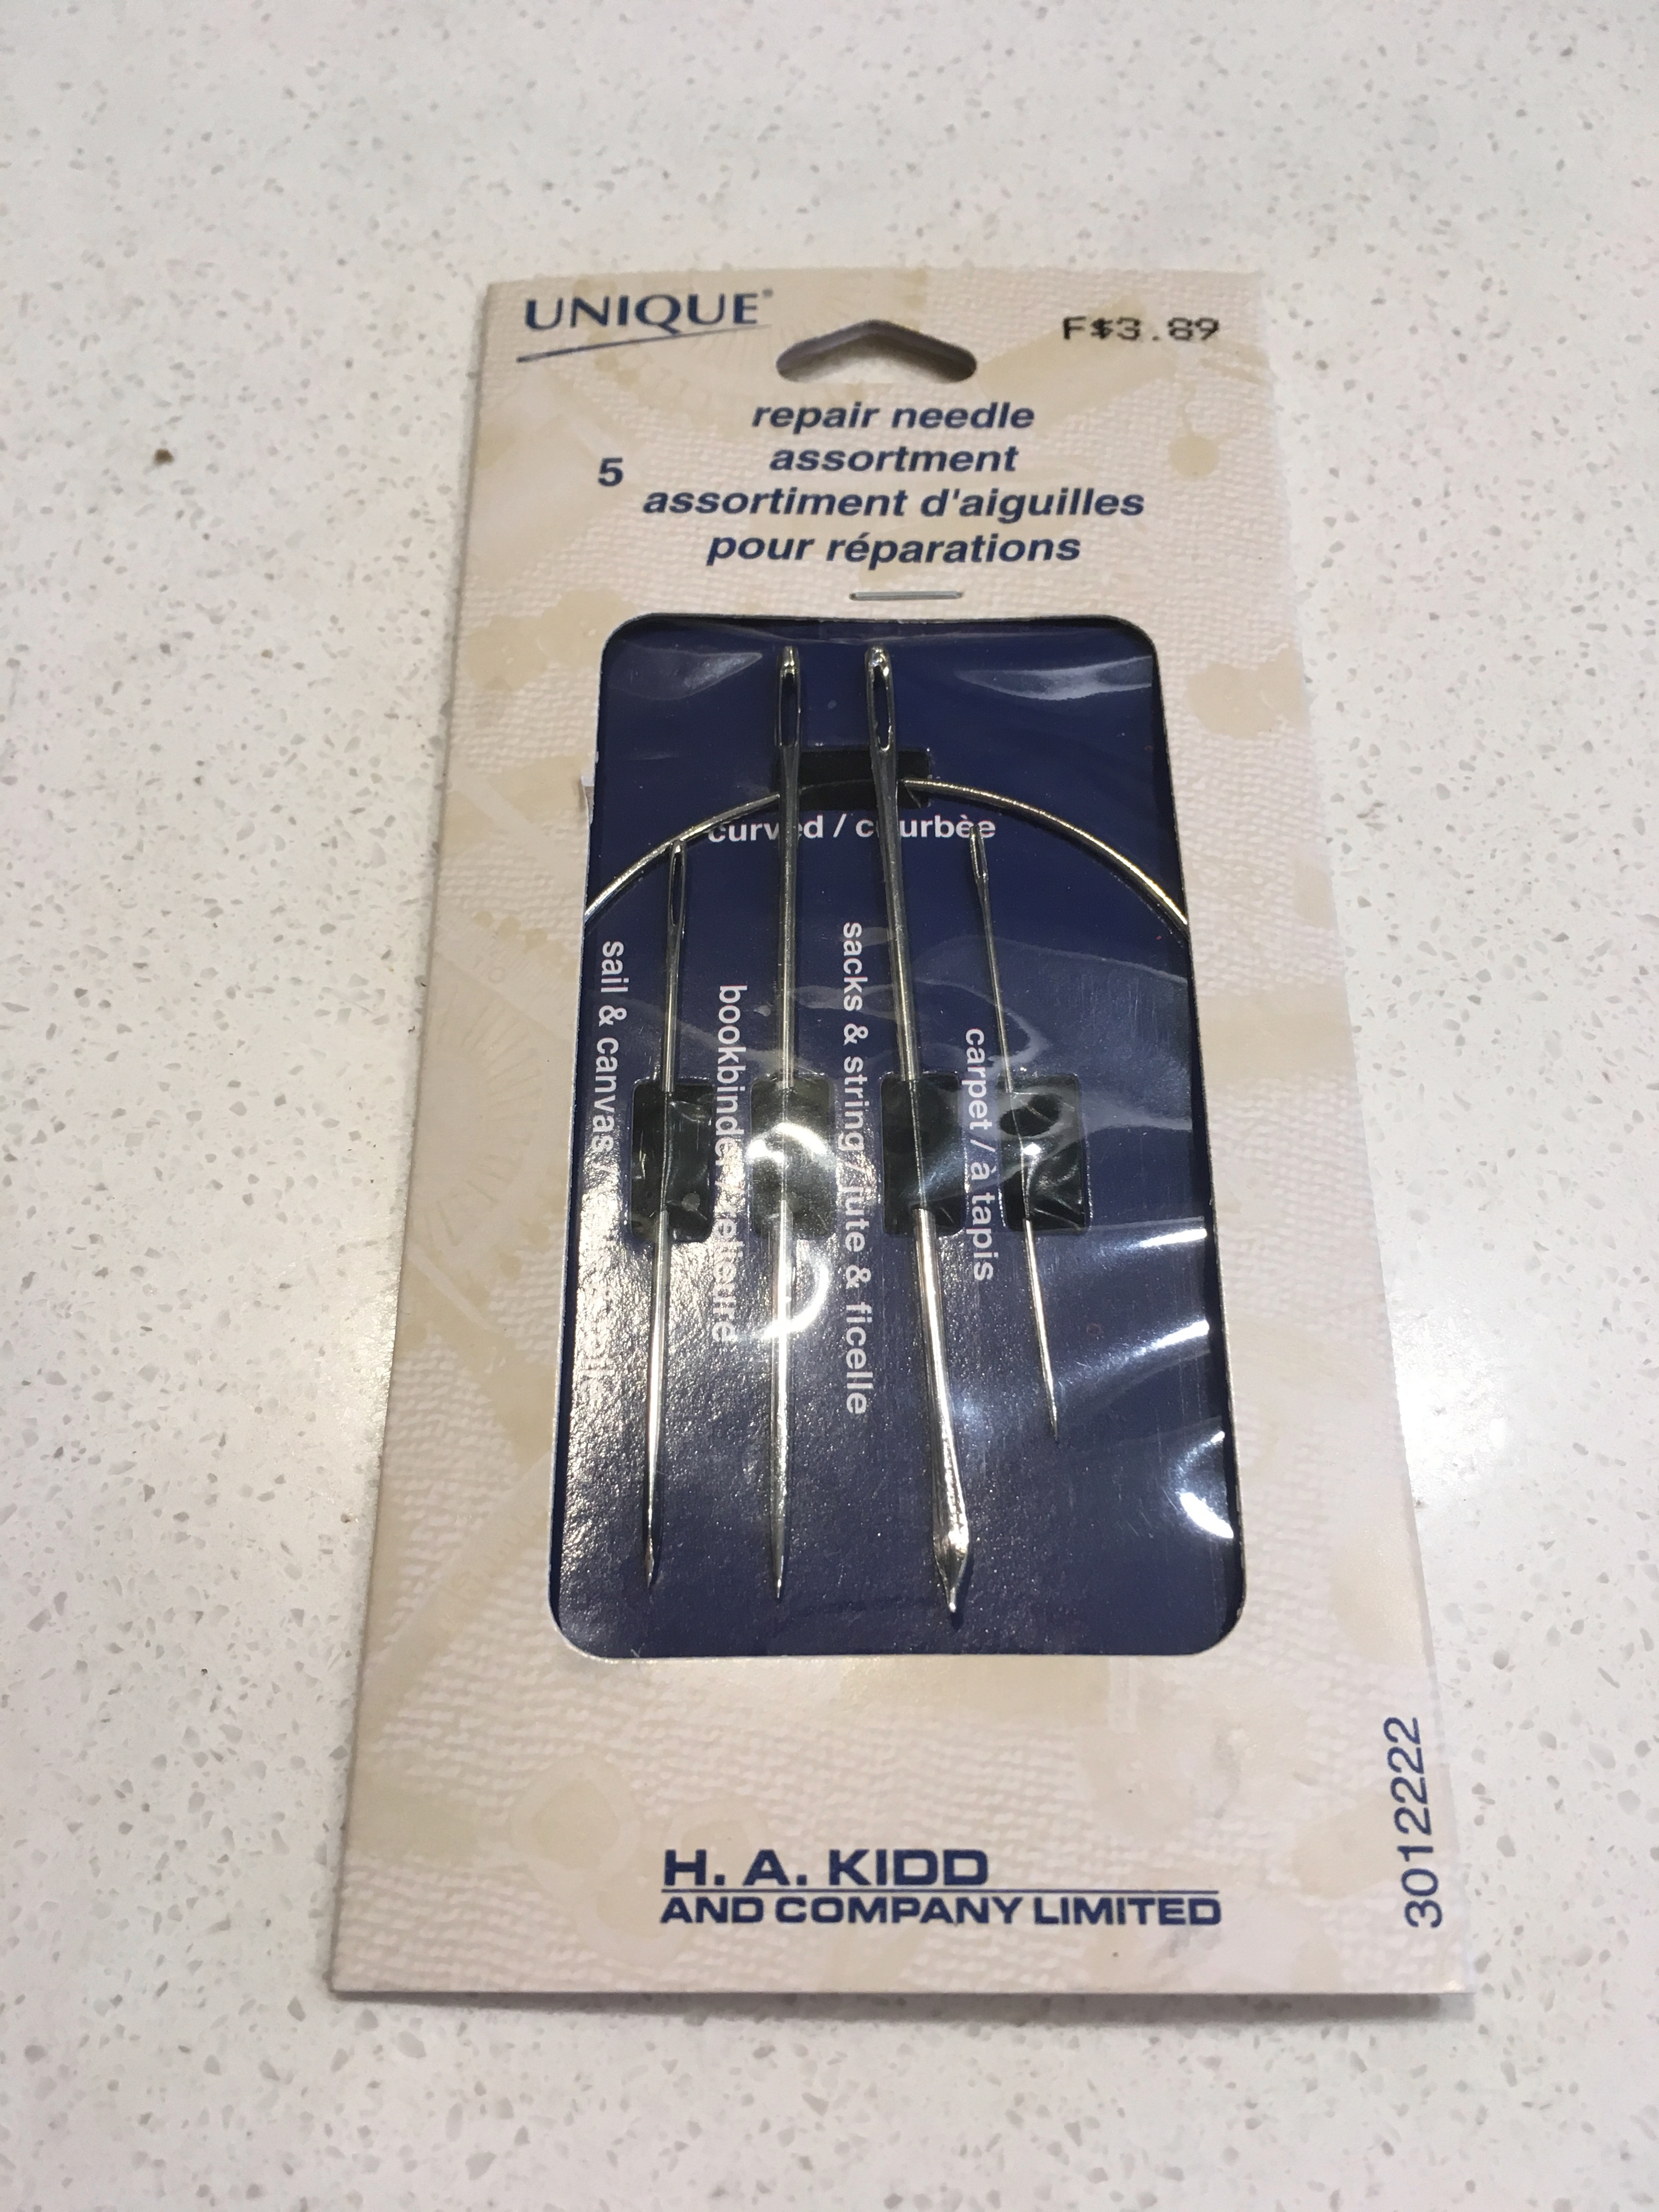
\includegraphics[width=0.25\textwidth]{\imageDir/\fileName/IMG_3206.jpg} &
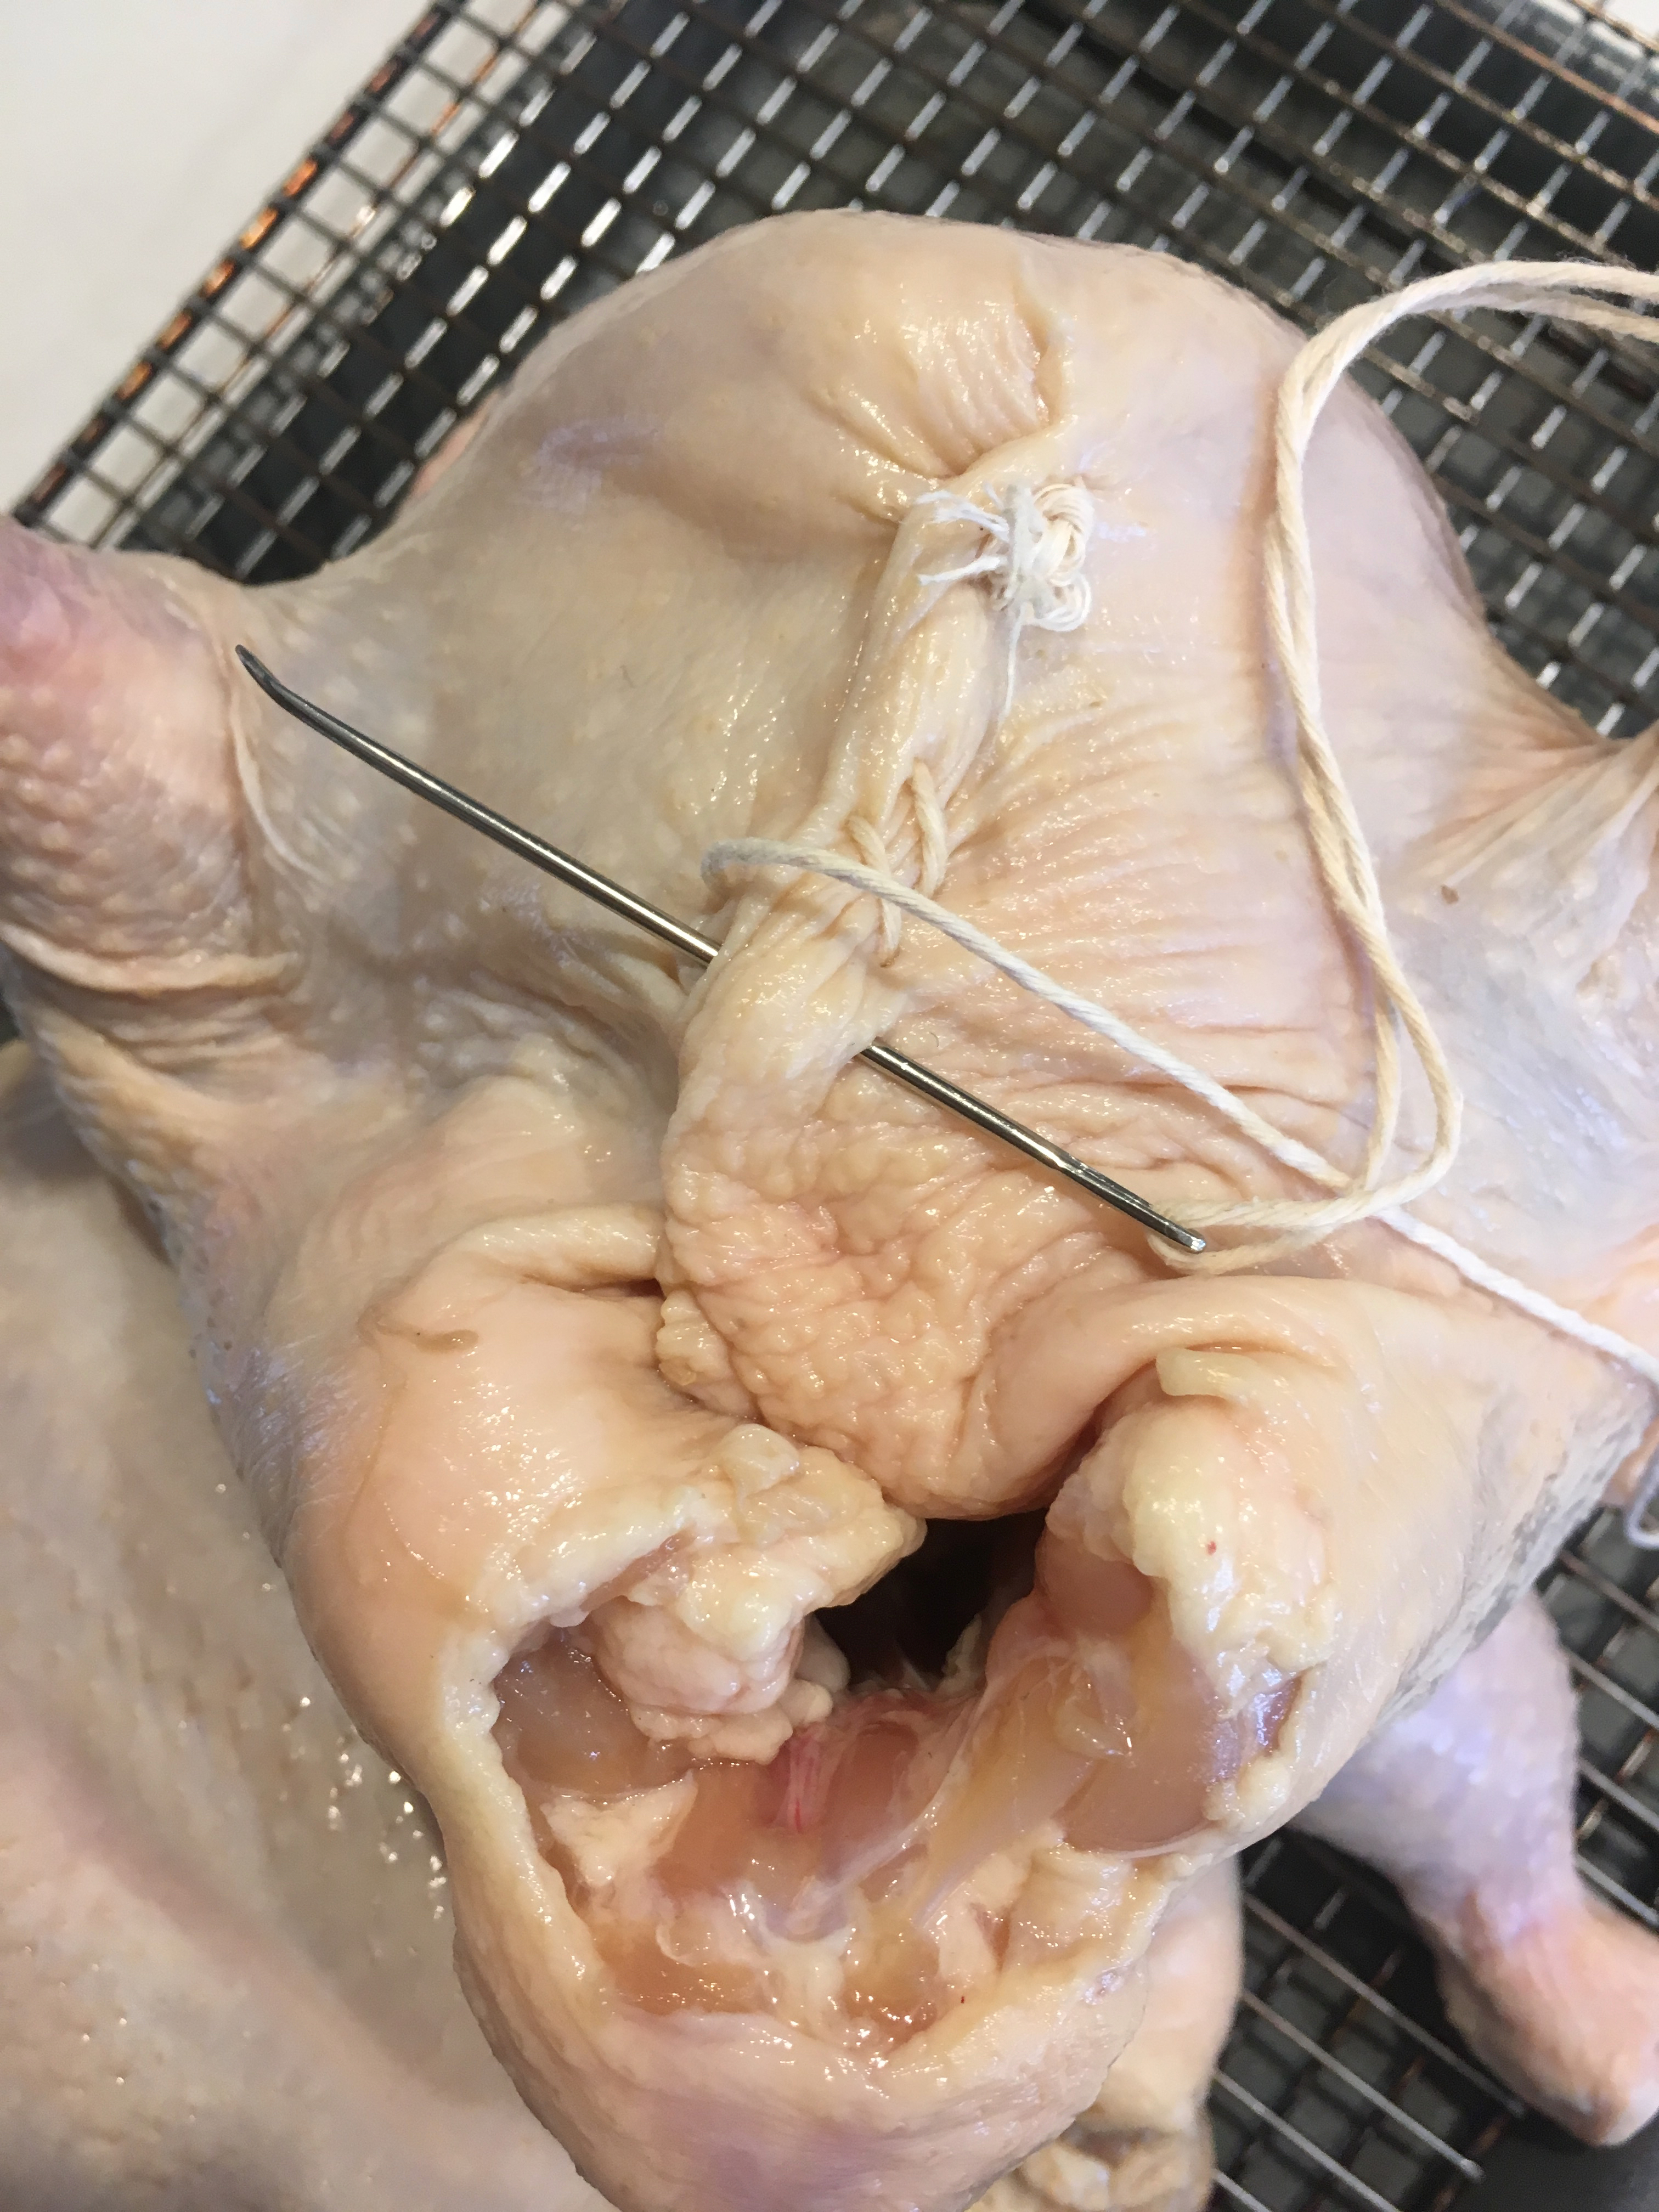
\includegraphics[width=0.25\textwidth]{\imageDir/\fileName/IMG_3214.jpg} &
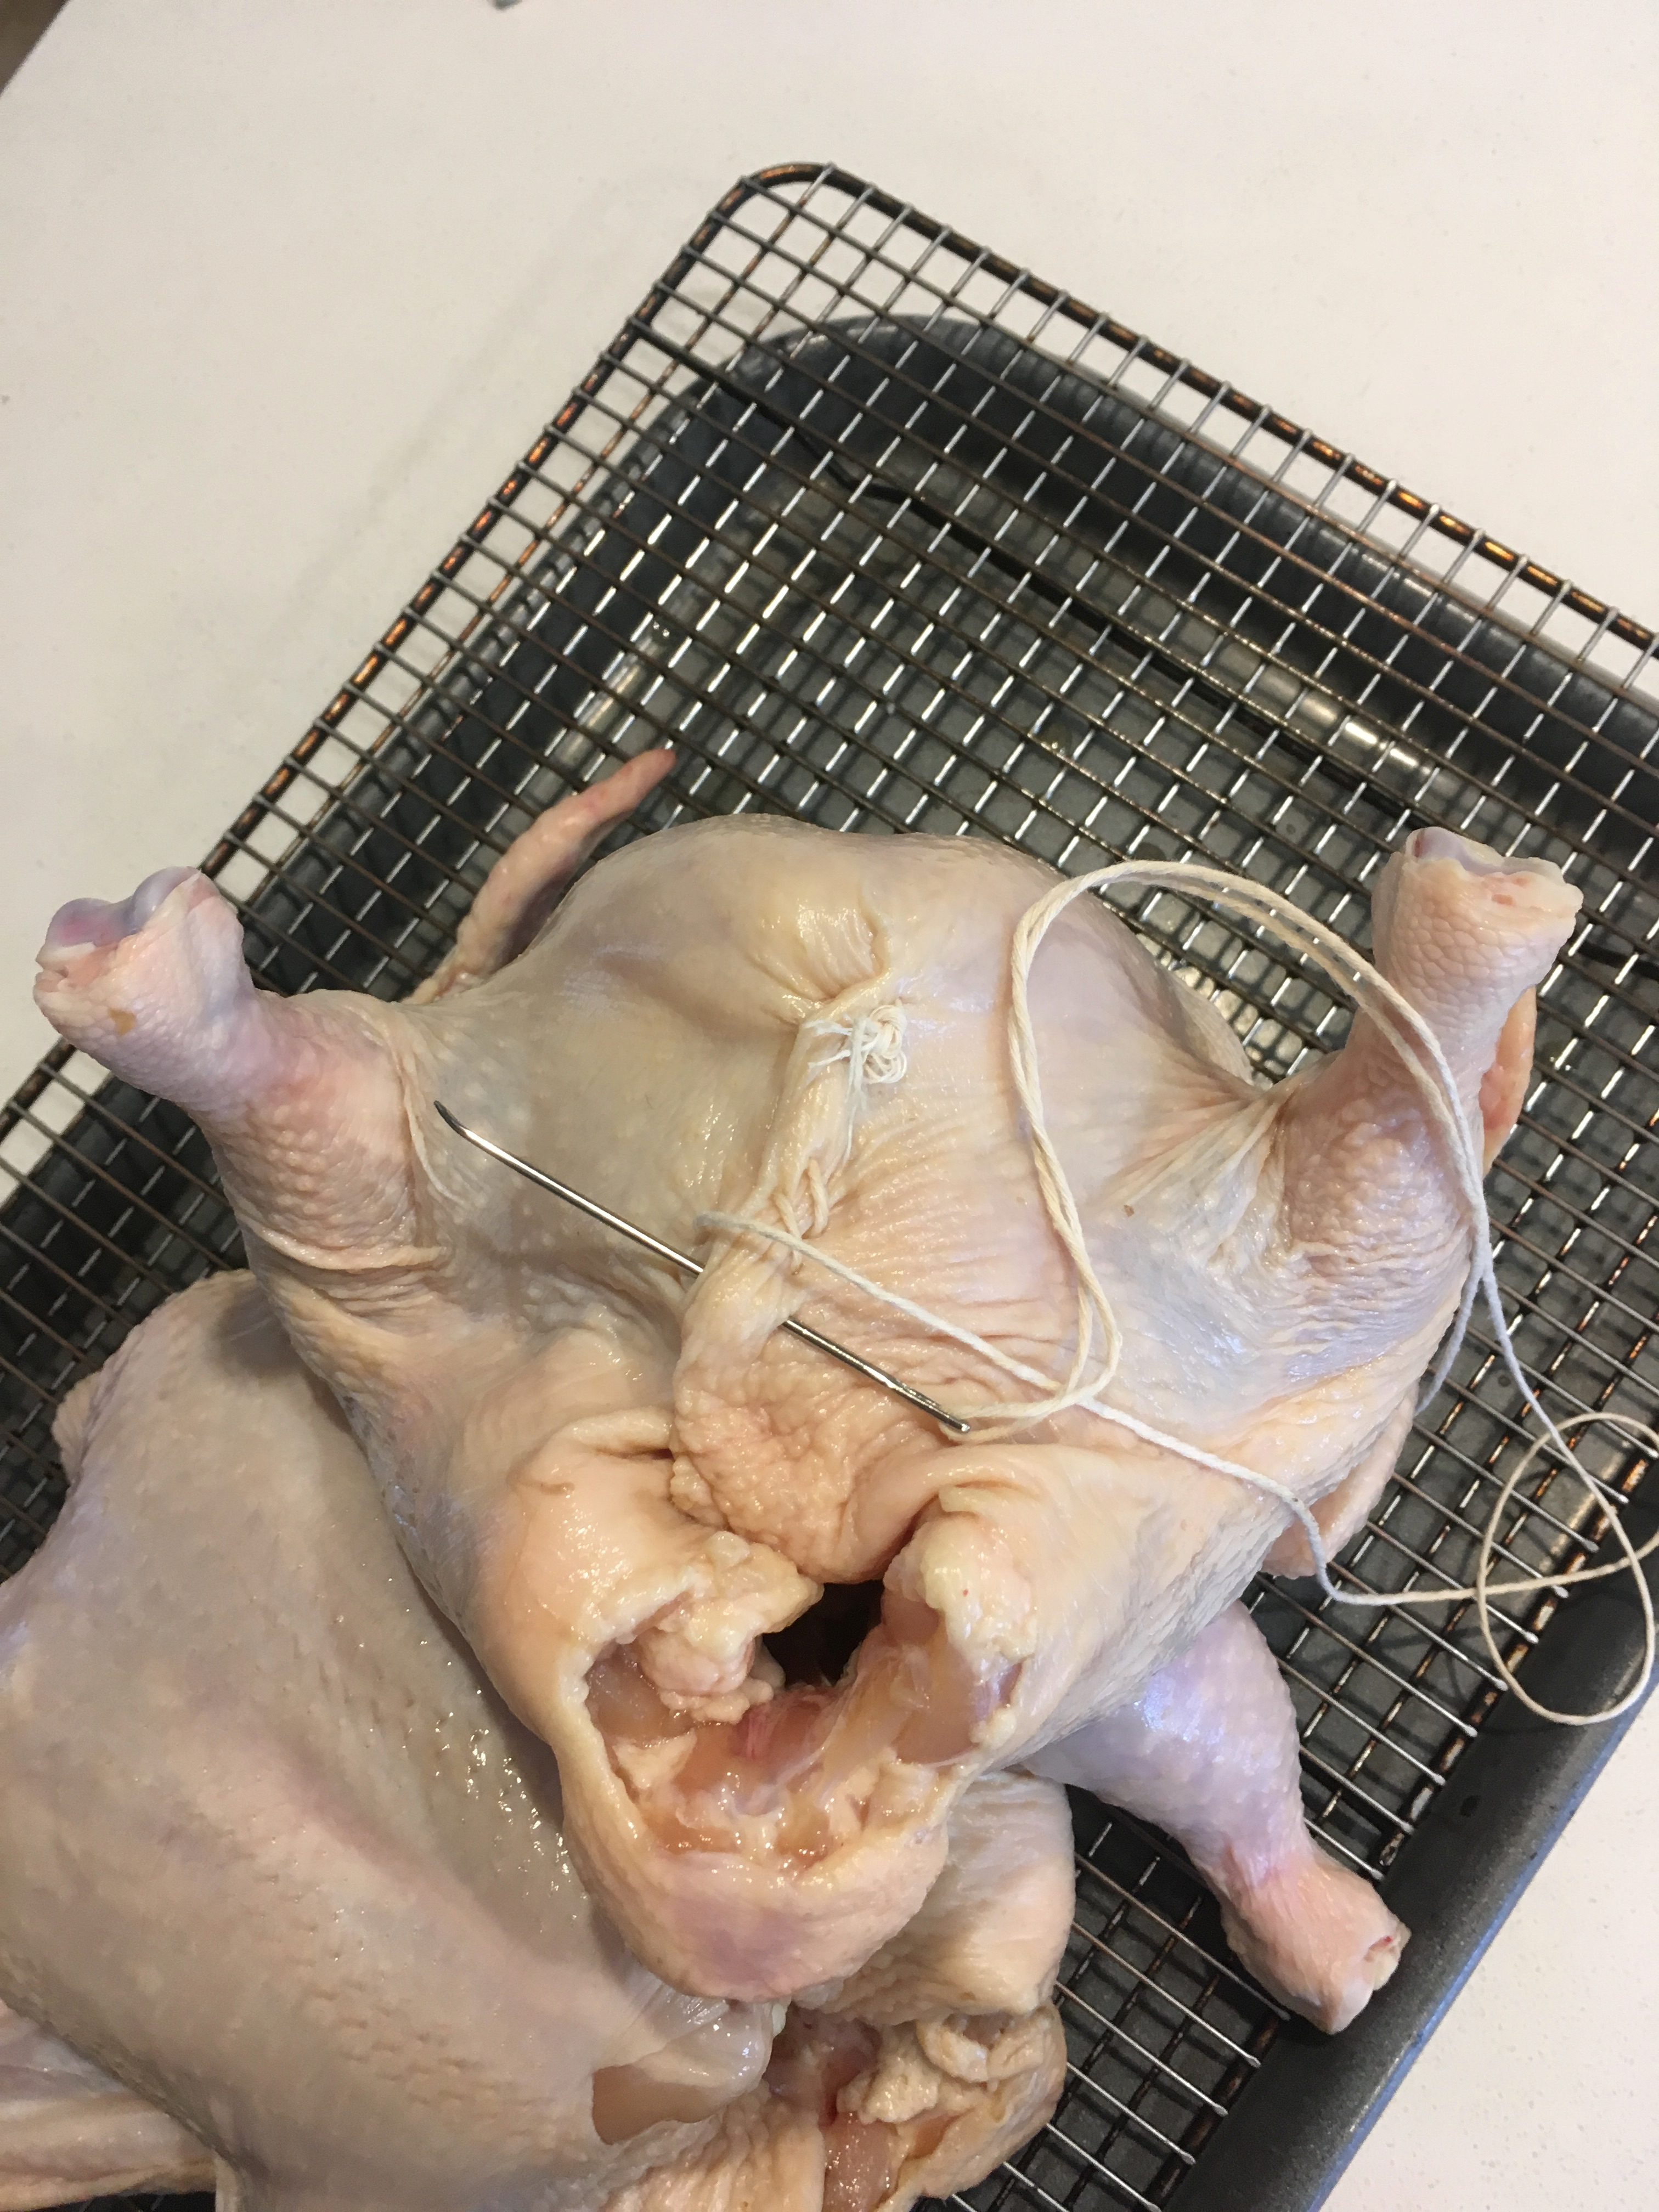
\includegraphics[width=0.25\textwidth]{\imageDir/\fileName/IMG_3216.jpg} \\
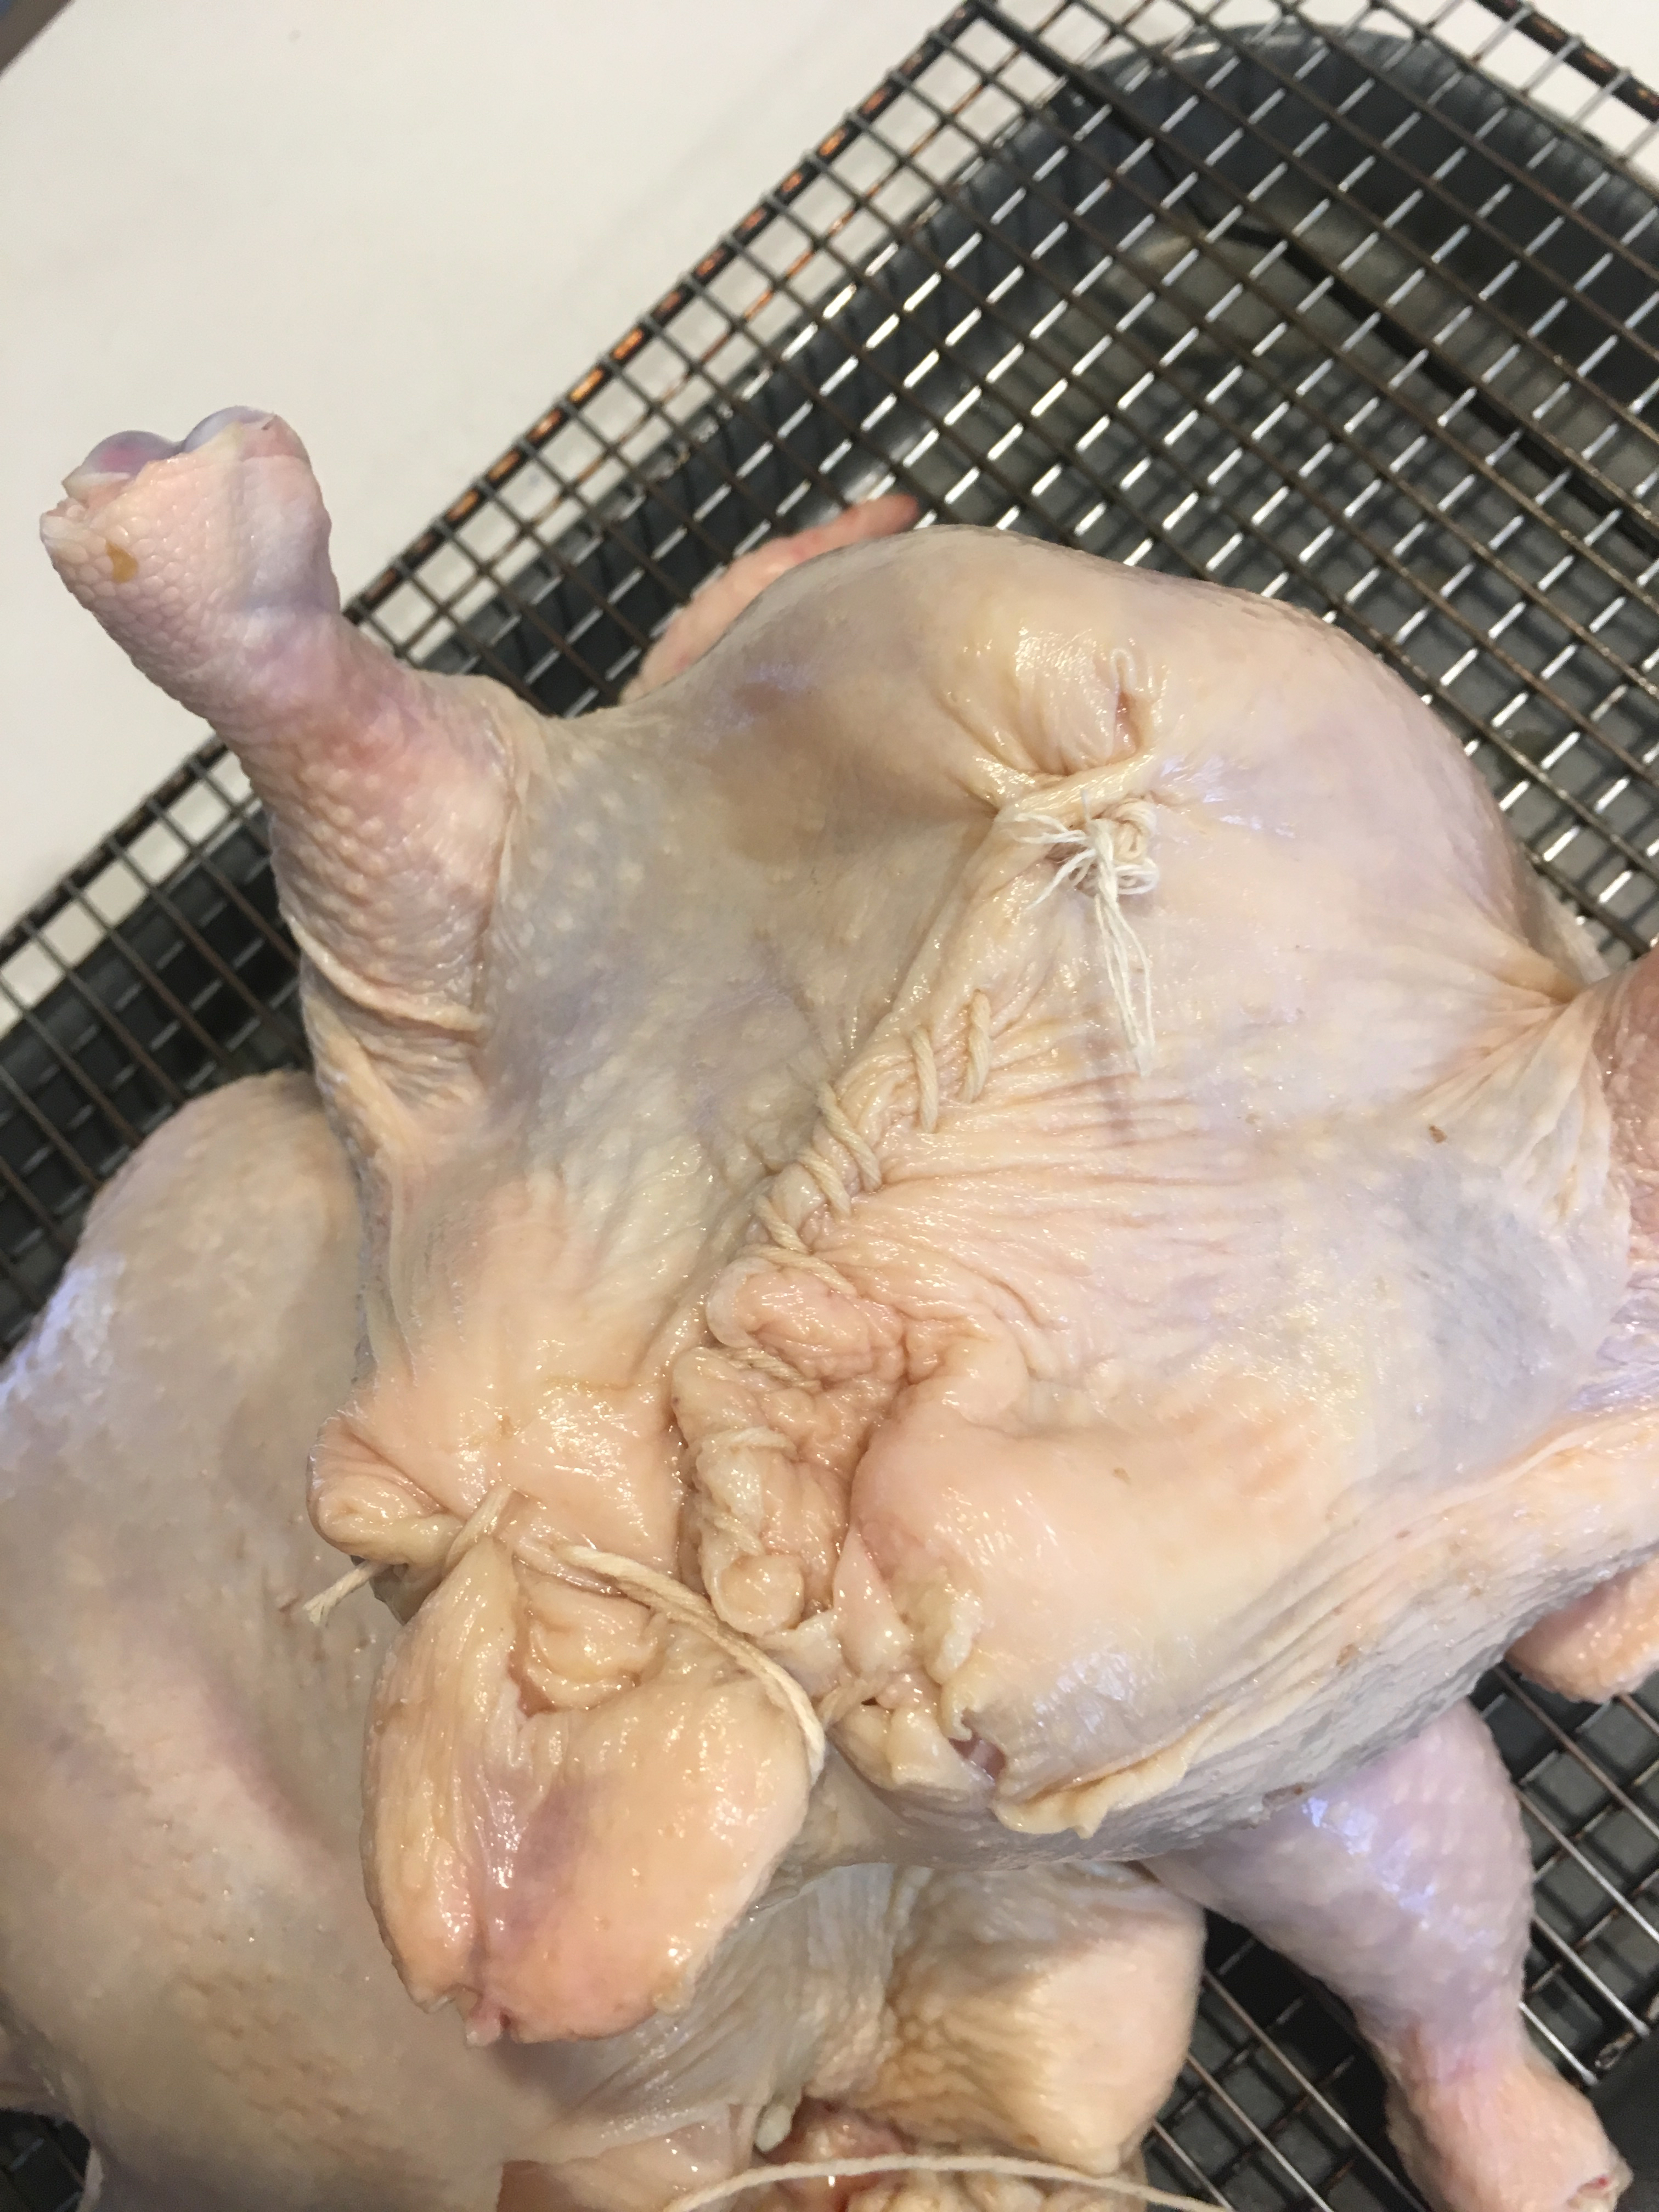
\includegraphics[width=0.25\textwidth]{\imageDir/\fileName/IMG_3217.jpg} &
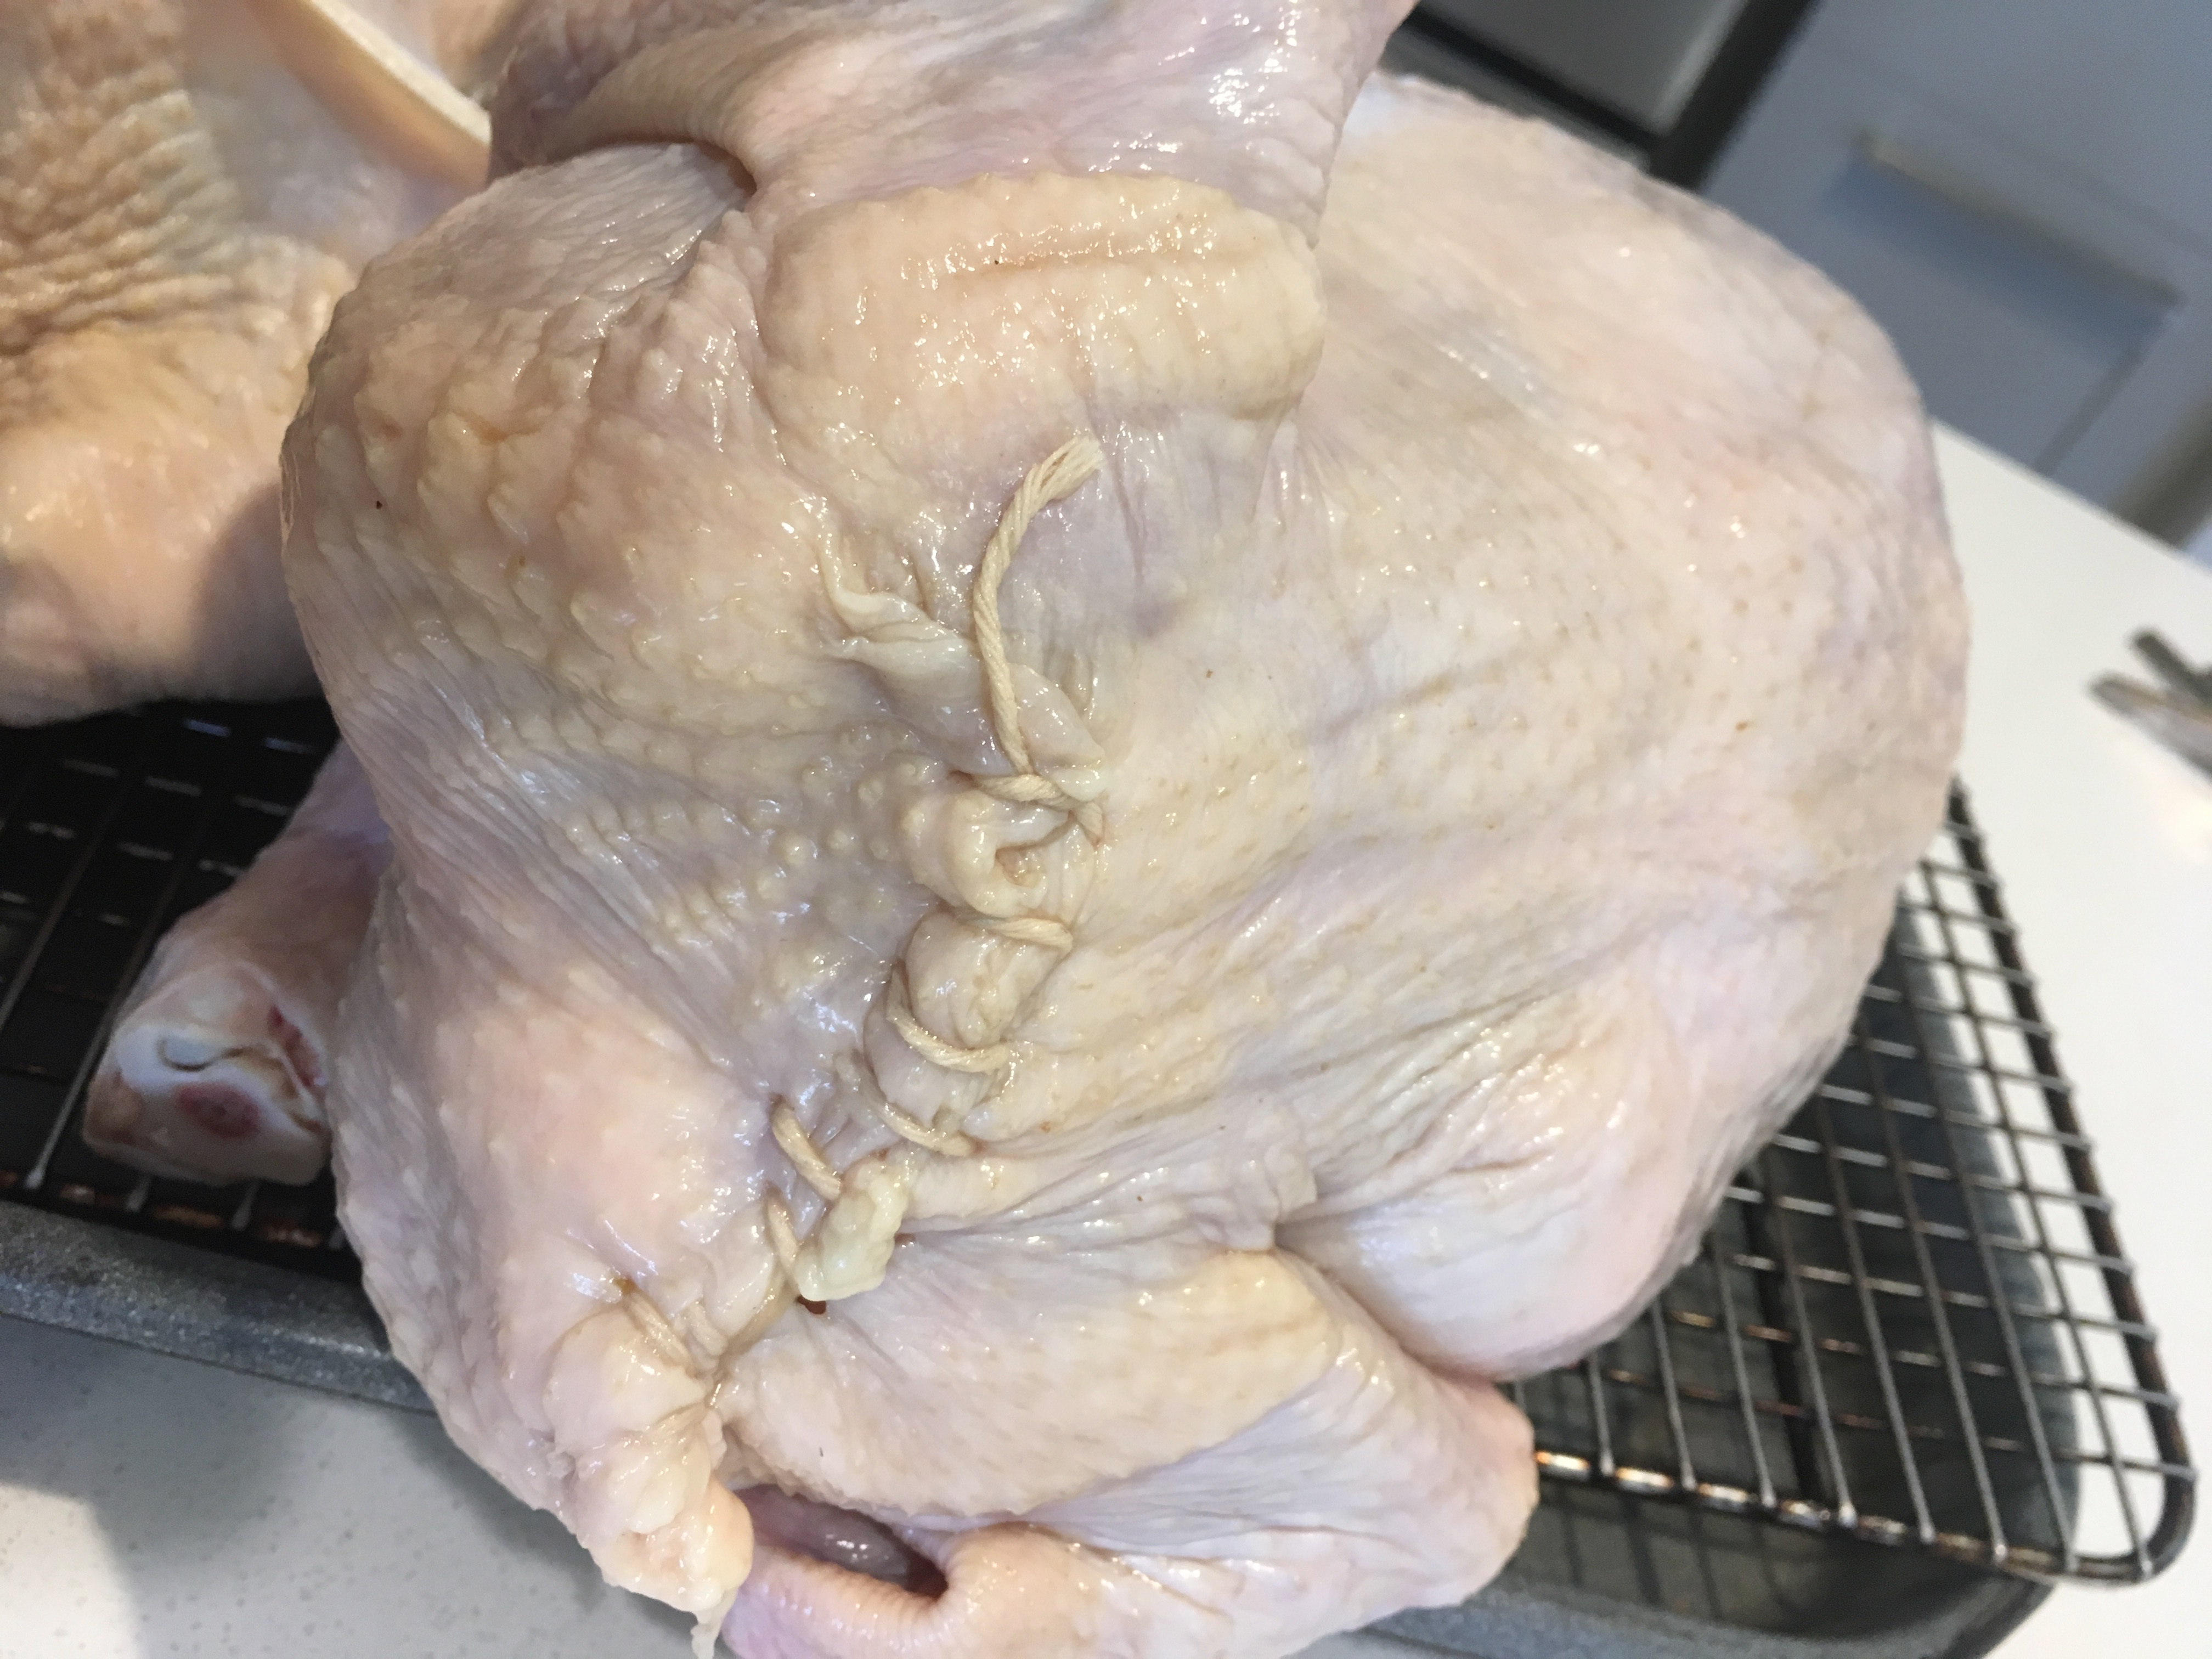
\includegraphics[width=0.25\textwidth]{\imageDir/\fileName/IMG_3218.jpg} &
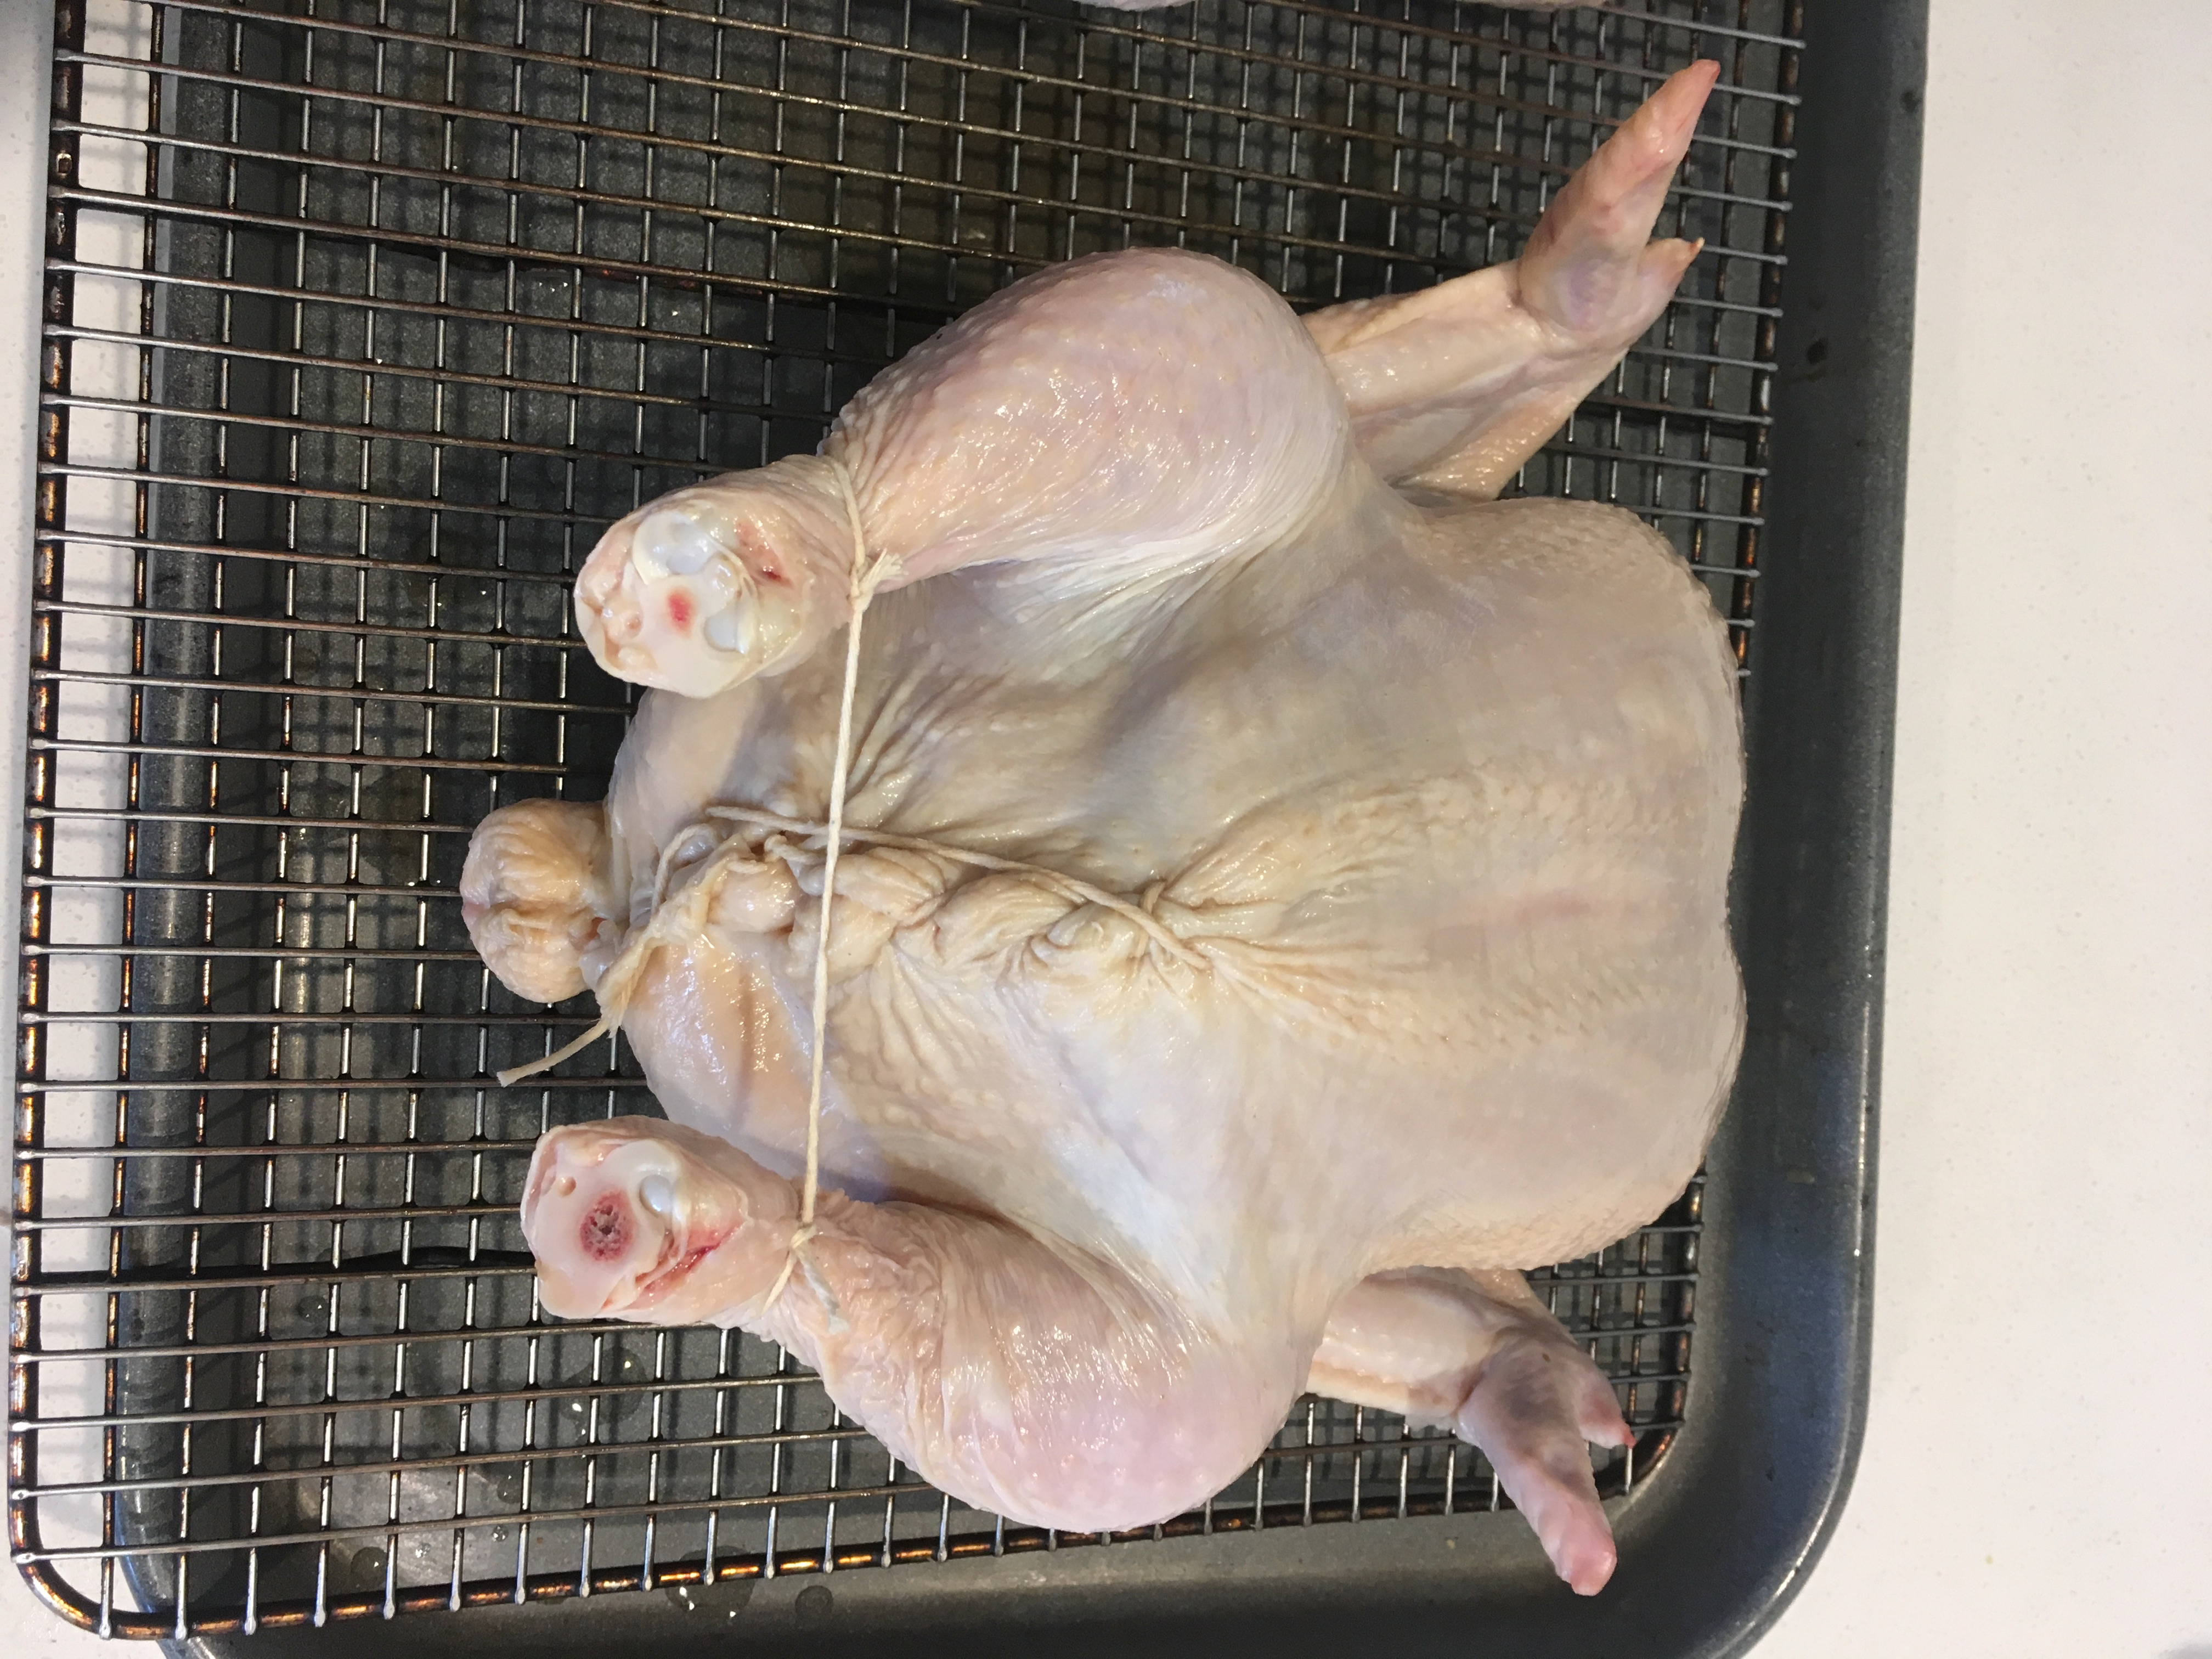
\includegraphics[width=0.25\textwidth]{\imageDir/\fileName/IMG_3219.jpg} \\
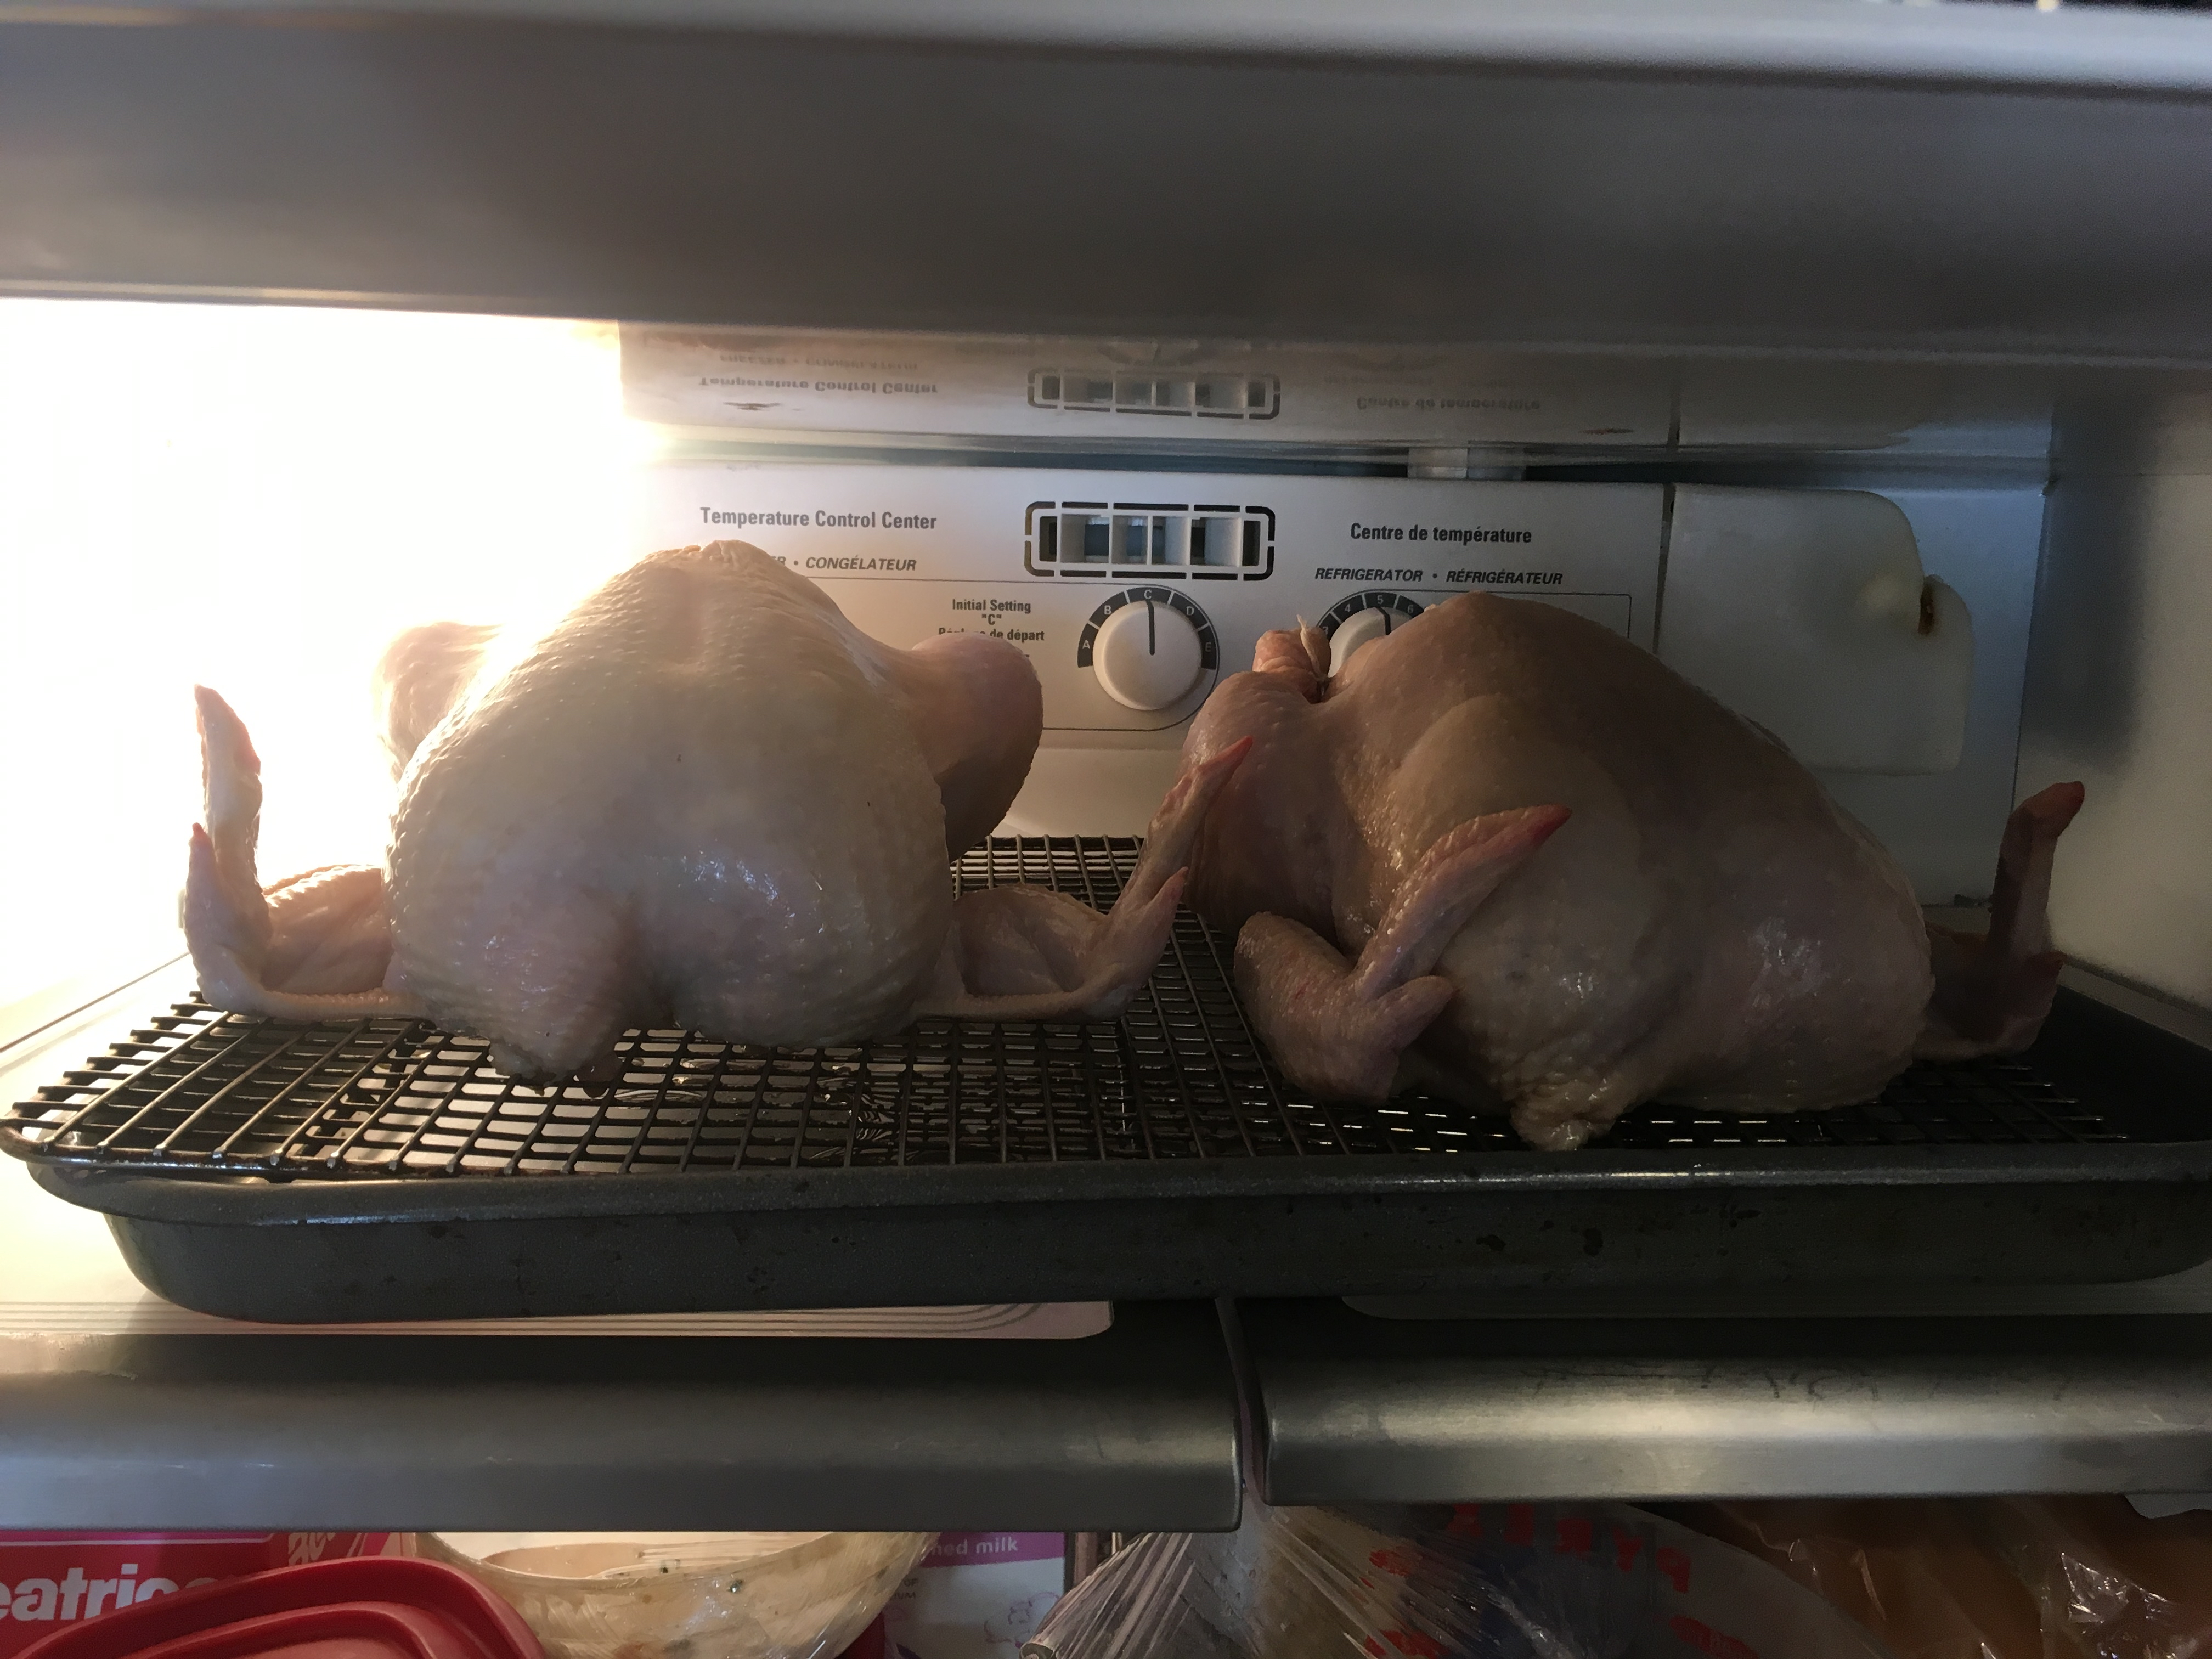
\includegraphics[width=0.25\textwidth]{\imageDir/\fileName/IMG_3220.jpg} &
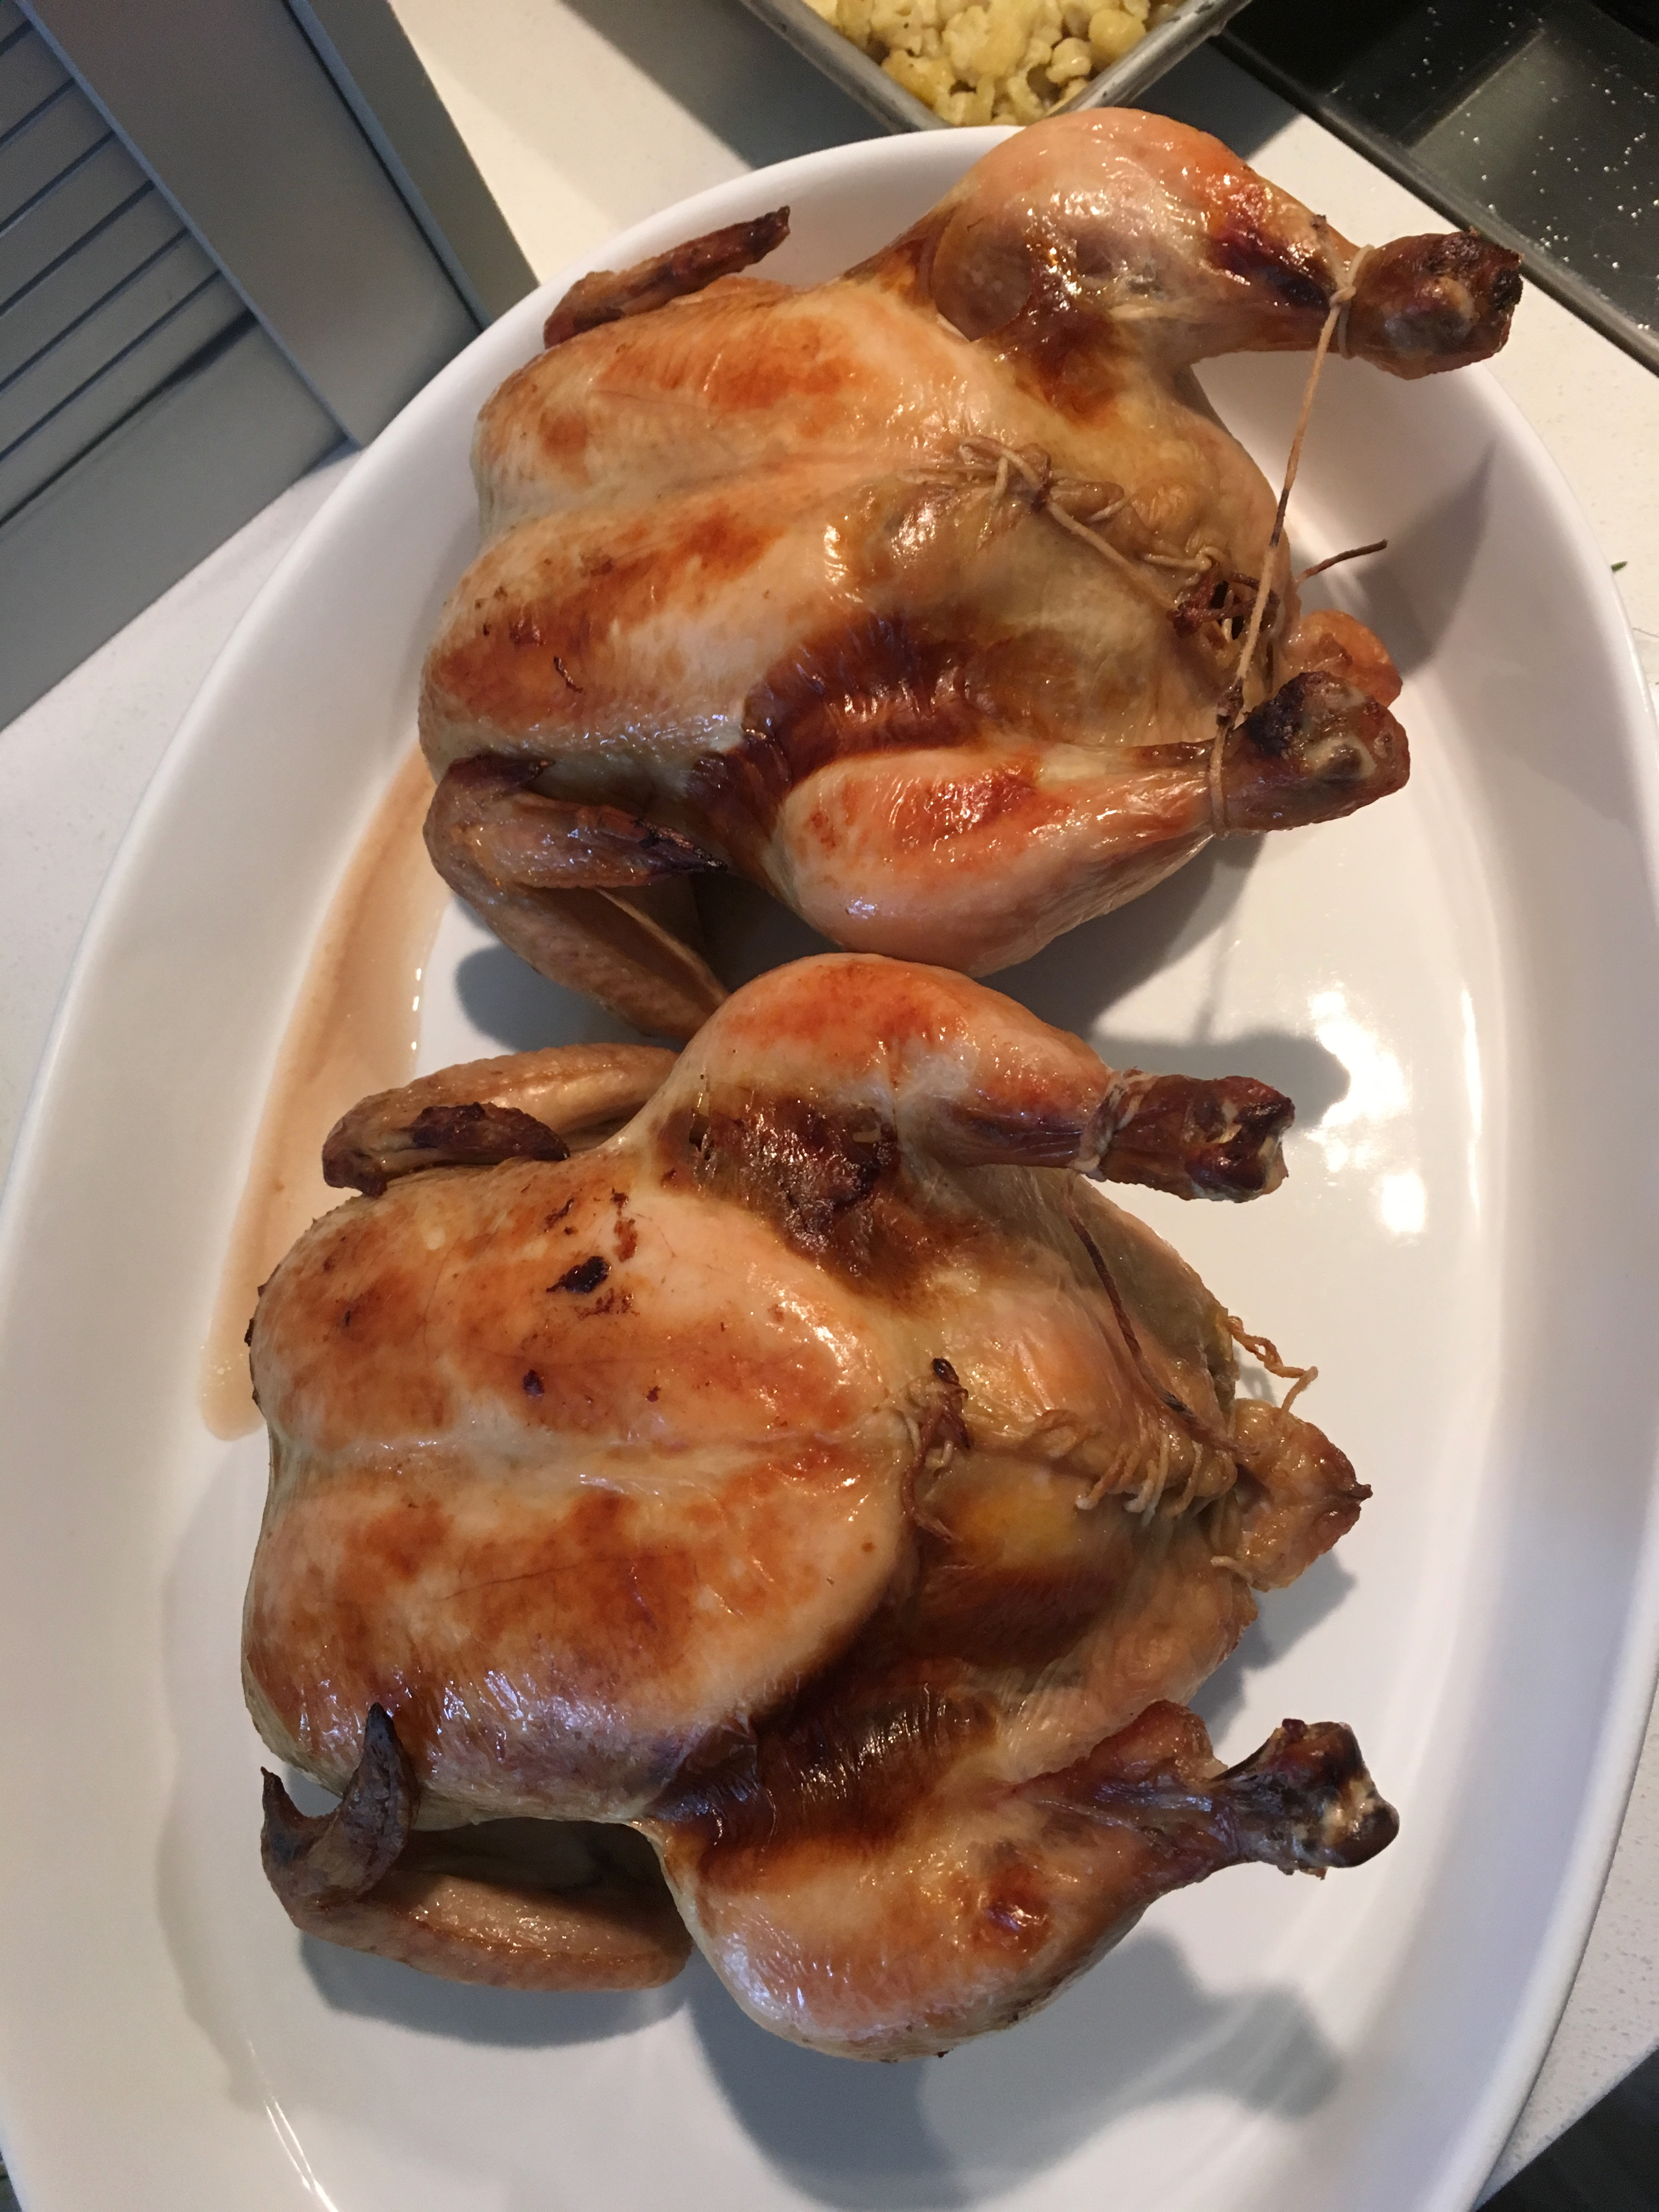
\includegraphics[width=0.25\textwidth]{\imageDir/\fileName/IMG_3228.jpg} \\
\end{tabular}
\end{table}

\end{document}



